\chapter{Empirical Results and Discussion}
\label{chap:empirical_results}

This chapter presents the empirical findings in a cumulative sequence: baseline treatment estimates, dynamic effects, robustness diagnostics, heterogeneity patterns, and mechanism evidence. The analysis asks not only whether an effect exists, but also when it emerges, where it is strongest, and through which channels it operates. This structure follows current reporting standards in causal empirical research.

The interpretive logic is sequential and cross-validating. Baseline estimates establish existence and magnitude; event studies test timing plausibility; falsification and sensitivity analyses test robustness; heterogeneity results identify boundary conditions; and mechanism regressions test channel coherence. This layered approach reduces reliance on any single coefficient and strengthens substantive inference through convergence across diagnostics.

\section{Baseline Regression Results}

This section establishes the benchmark effect size and statistical reliability of MSCI inclusion under nested DID specifications. By comparing parsimonious and fully controlled models, it assesses sensitivity to covariate structure and fixed-effect saturation while maintaining a clear distinction between statistical significance and economic magnitude.

\subsection{Main Effect: MSCI Inclusion Increases DT\_Comp by 0.39 Log Points ($\approx$48\%)}

The central empirical question is whether MSCI inclusion produces a statistically and economically meaningful rise in corporate digital transformation after controlling for firm-specific characteristics and common time shocks. Equation~(\ref{eq:twfe_did}) provides the main estimate by exploiting the quasi-experimental timing of phased MSCI inclusion, with firm and year fixed effects absorbing persistent firm differences and aggregate shocks. To assess specification sensitivity, three nested models are estimated: a parsimonious FE model, a preferred model with the full time-varying control set from Chapter~\ref{chap:research_design_1}, and a fully saturated model with industry-by-year and province-by-year interactions.

\begin{table}[htbp]
\centering
\caption{Baseline Difference-in-Differences Estimates}
\label{tab:baseline_did}
\small
\begin{tabular}{lccc}
\toprule
\textbf{Variable} & \textbf{(1) DT} & \textbf{(2) DT} & \textbf{(3) DT} \\
\midrule
MSCI $\times$ Post & 0.705*** (0.038) & 0.394*** (0.039) & 0.044 (0.030) \\
Size & & 0.260*** (0.009) & 0.232*** (0.008) \\
ROA & & $-$0.123*** (0.016) & $-$0.019*** (0.007) \\
ROE & & 0.005 (0.014) & $-$0.000 (0.005) \\
CashFlow & & 0.175*** (0.009) & 0.024*** (0.007) \\
Leverage & & $-$0.264*** (0.008) & $-$0.075*** (0.007) \\
TobinQ & & 0.006 (0.017) & $-$0.006 (0.007) \\
Ownership & & $-$0.225*** (0.008) & $-$0.054*** (0.006) \\
BoardSize & & $-$0.003 (0.007) & 0.039*** (0.006) \\
FirmAge & & $-$0.089*** (0.008) & $-$0.057*** (0.007) \\
Firm-FE & Yes & Yes & Yes \\
Year-FE & Yes & Yes & Yes \\
Industry $\times$ Year FE & No & No & Yes \\
Province $\times$ Year FE & No & No & Yes \\
$N$ & 34,503 & 34,503 & 34,503 \\
$R^2$ & 0.010 & 0.091 & 0.504 \\
\bottomrule
\end{tabular}
\begin{tablenotes}
\small
\item \textit{Notes:} Dependent variable is DT Index (log-transformed), $DT\_Comp = \log(1 + \Sigma\;\mathrm{keywords})$. Coefficients are in log points; to convert to percentage effects, use $\exp(\beta) - 1$. Column~(1) is the baseline without controls; Column~(2) is the preferred specification with full controls; Column~(3) includes high-dimensional interactive fixed effects and is interpreted as a conservative lower bound. Robust standard errors clustered at the firm level. Significance: *** $p < 0.01$, ** $p < 0.05$, * $p < 0.10$.
\end{tablenotes}
\end{table}

The estimates in Table~\ref{tab:baseline_did} compare the three baseline DID models. Column~(1), which includes firm and year fixed effects but no time-varying controls, yields a coefficient of 0.705 ($\mathrm{s.e.} = 0.038$, $p < 0.001$), equivalent to about $\exp(0.705)-1 \approx 102\%$ in the log-transformed digital-transformation index.

Adding rich time-varying controls in Column~(2) reduces the coefficient to 0.394 ($\mathrm{s.e.} = 0.039$, $p < 0.001$). This is the preferred specification because it balances covariate adjustment with preservation of meaningful treatment variation; the implied effect is $\exp(0.394)-1 \approx 48\%$. Column~(3) adds industry$\times$year and province$\times$year fixed effects and returns a smaller, statistically insignificant estimate (0.044; $\mathrm{s.e.} = 0.030$). We interpret Column~(3) as a conservative lower-bound diagnostic: because MSCI eligibility is correlated with industry composition, high-dimensional interactions may absorb part of the treatment-induced variation.

\subsection{Stability Across Specifications and Control Sets}

Key control variable coefficients align with theoretical expectations throughout. Firm size (log assets) enters positively (0.260 and 0.232 in columns 1 and 2), consistent with scale economies in digital investment. Leverage enters negatively ($-$0.264 and $-$0.075), confirming that financially constrained firms invest less in digital transformation. Cash flow enters positively (0.175 and 0.024), supporting the internal financing channel. Importantly, the sign stability of core controls across nested specifications suggests that the baseline treatment coefficient is not being generated by unstable model fit or extreme sensitivity to covariate inclusion.

\subsection{Economic Interpretation and Practical Significance}

At the control group mean of 12.78 keywords, the preferred estimate of 0.394 log points corresponds to an increase of approximately 6.0 additional keywords in annual report digital transformation language---moving a median treated firm from the 50th to roughly the 60th percentile of the pre-treatment distribution. This magnitude is economically significant, representing approximately half a within-firm standard deviation and a multiple of the control group's 4\% annual organic growth rate. In applied-policy terms, the result is large enough to indicate a substantive shift in strategic orientation rather than a negligible reporting adjustment.

\section{Event Study and Dynamic Treatment Effects}

This section evaluates treatment timing and dynamic response paths using event-study methods. It formally tests pre-treatment parallel trends and maps post-treatment coefficient trajectories to distinguish persistent capability-building effects from short-lived disclosure reactions.

\subsection{Mean Digital Transformation Outcomes for Treated vs.\ Control Firms}
Before turning to formal regression evidence, it is useful to examine the raw time-series trajectories of digital transformation for treated and control firms.

\begin{figure}[htbp]
\centering
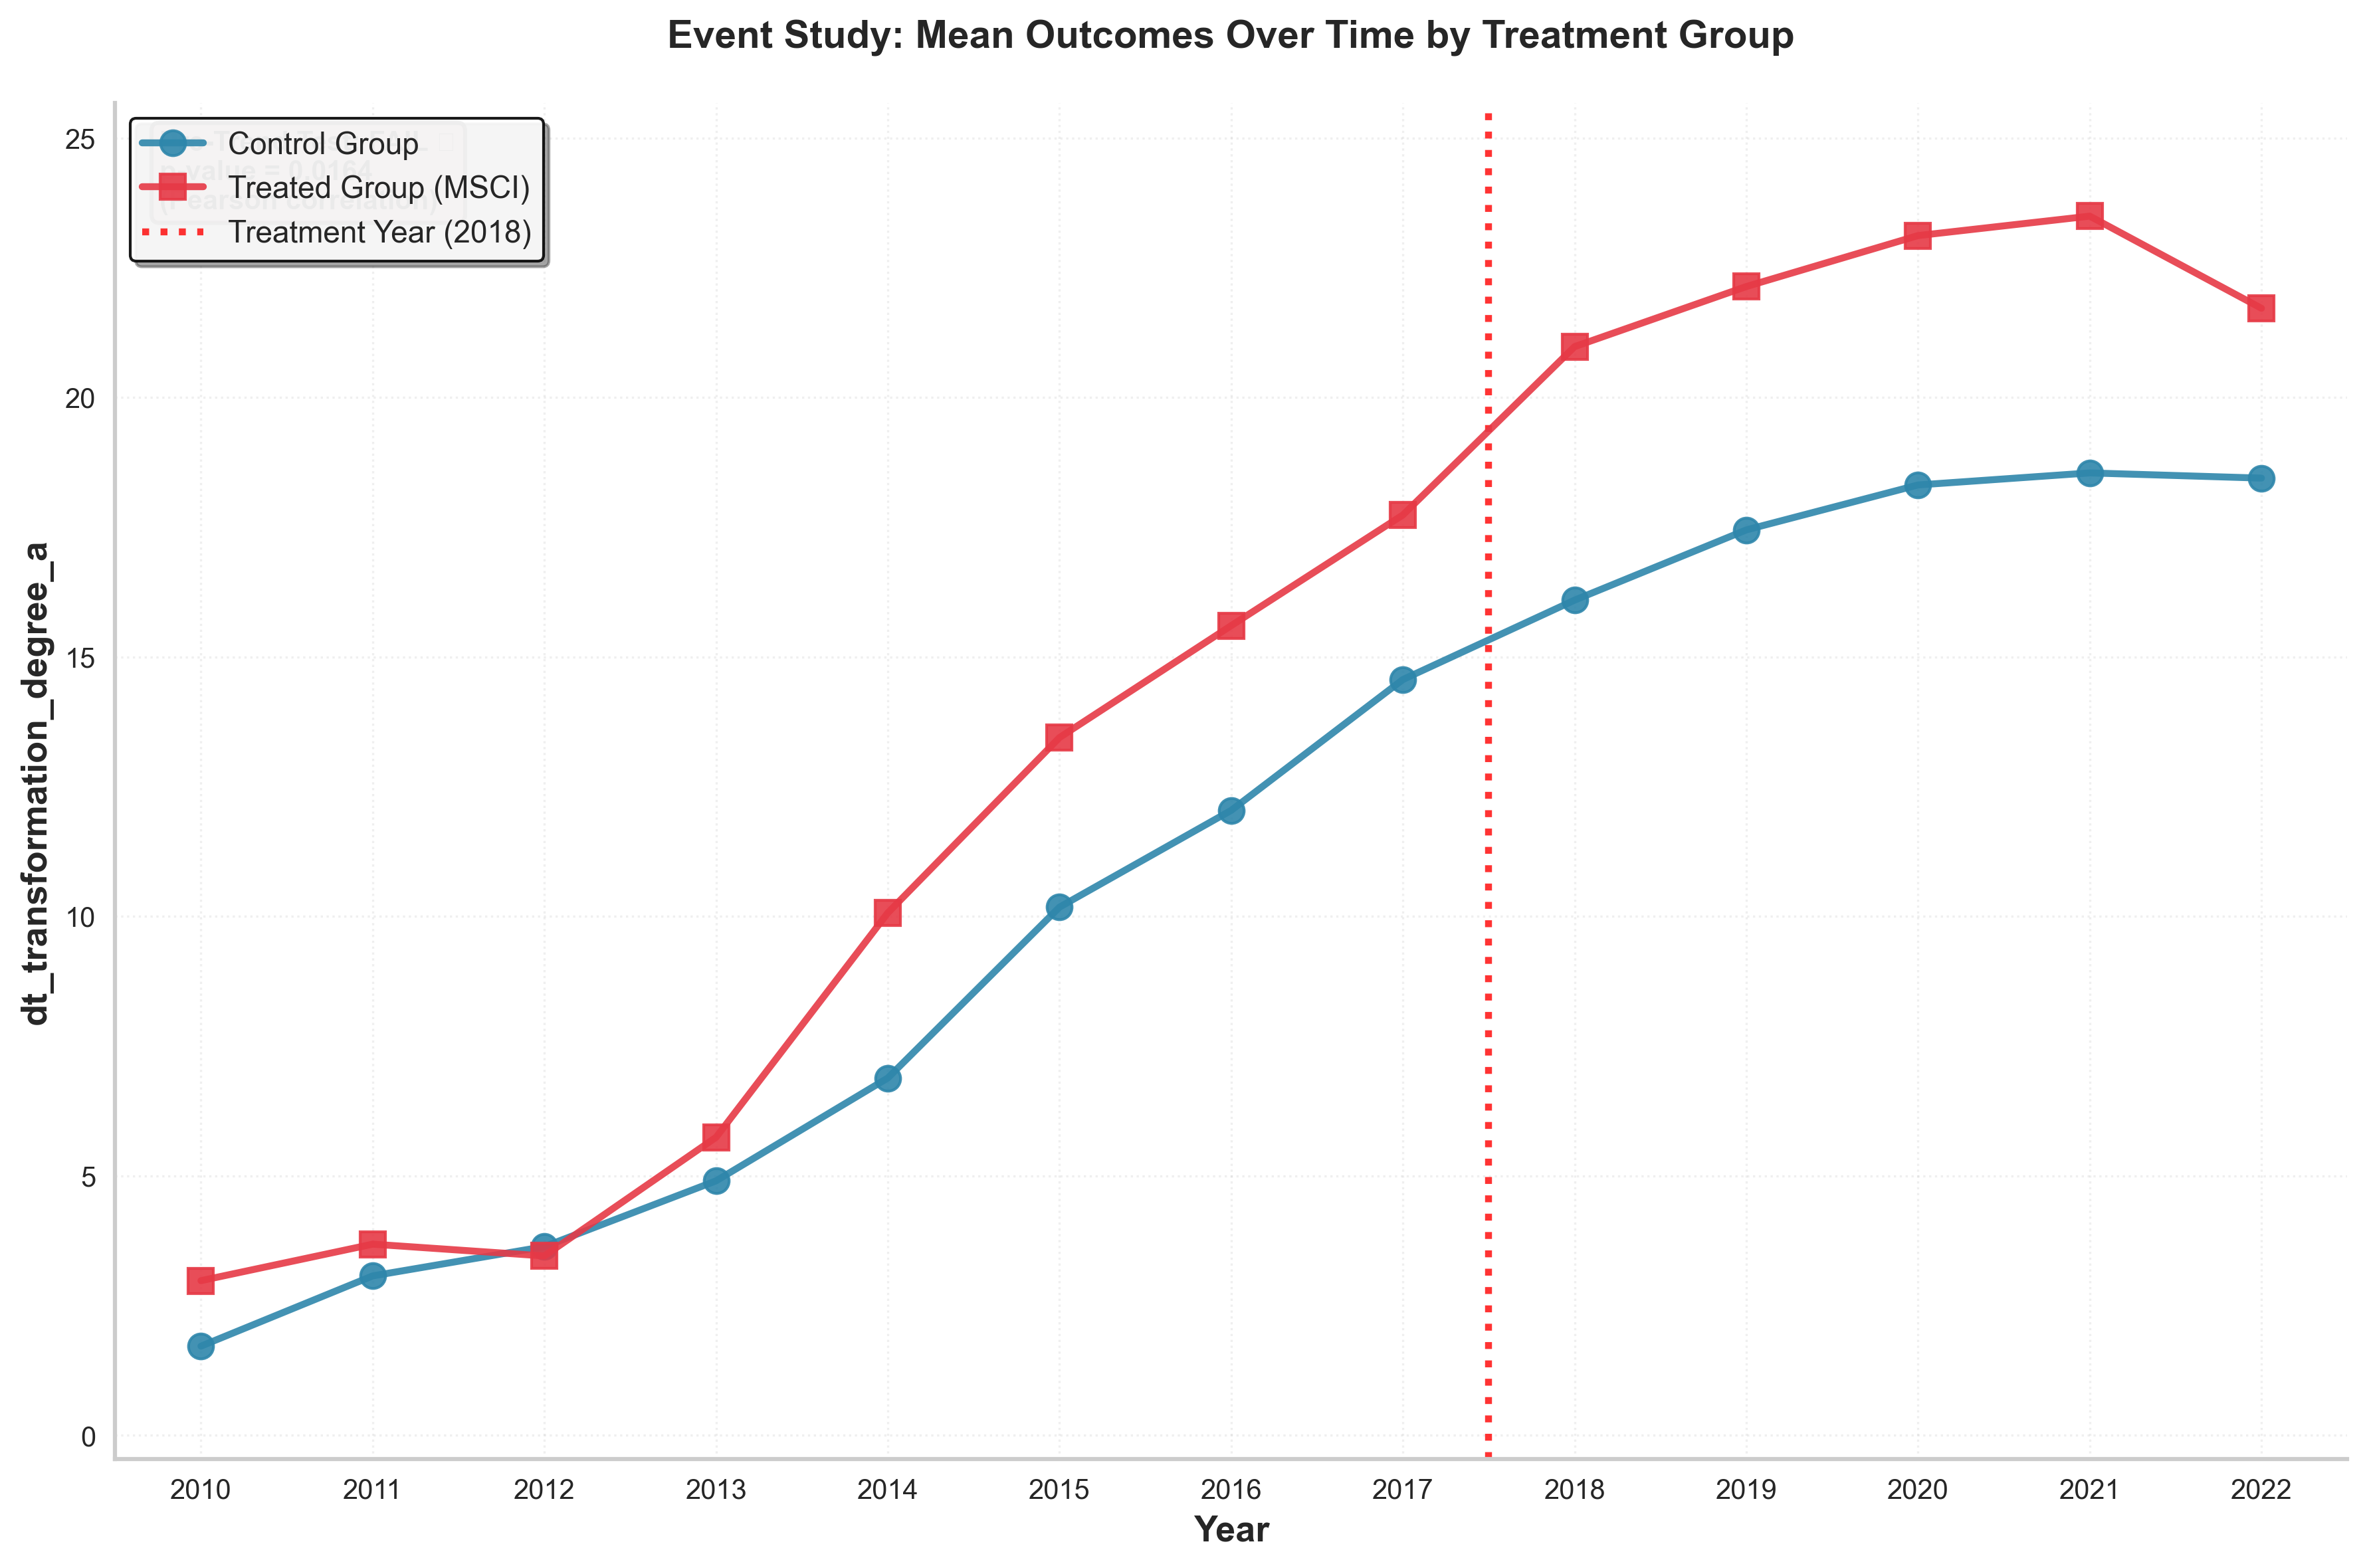
\includegraphics[width=0.8\textwidth]{figures/fig6_1_event_study.png}
\caption{Event Study: Mean Digital Transformation for Treated vs.\ Control Firms}
\label{fig:event_study}
\end{figure}

Figure~\ref{fig:event_study} displays mean digital transformation outcomes over time for the treatment and control groups. Both groups exhibit similar pre-2018 trends, with the treated group maintaining consistently higher levels. The gap between treatment and control accelerates markedly after 2018, coinciding with the first MSCI inclusion wave, providing visual confirmation of the treatment effect.

\subsection{Dynamic Treatment Effect Coefficients with 95\% Confidence Intervals}

Figure~\ref{fig:event_study} shows post-2018 divergence, but visual evidence alone cannot distinguish a true treatment shift from a pre-existing trend difference. Equation~(\ref{eq:event_study}) addresses this directly by estimating year-specific treatment coefficients $\delta_k$ relative to the omitted reference year $k=-1$.

\begin{figure}[htbp]
\centering
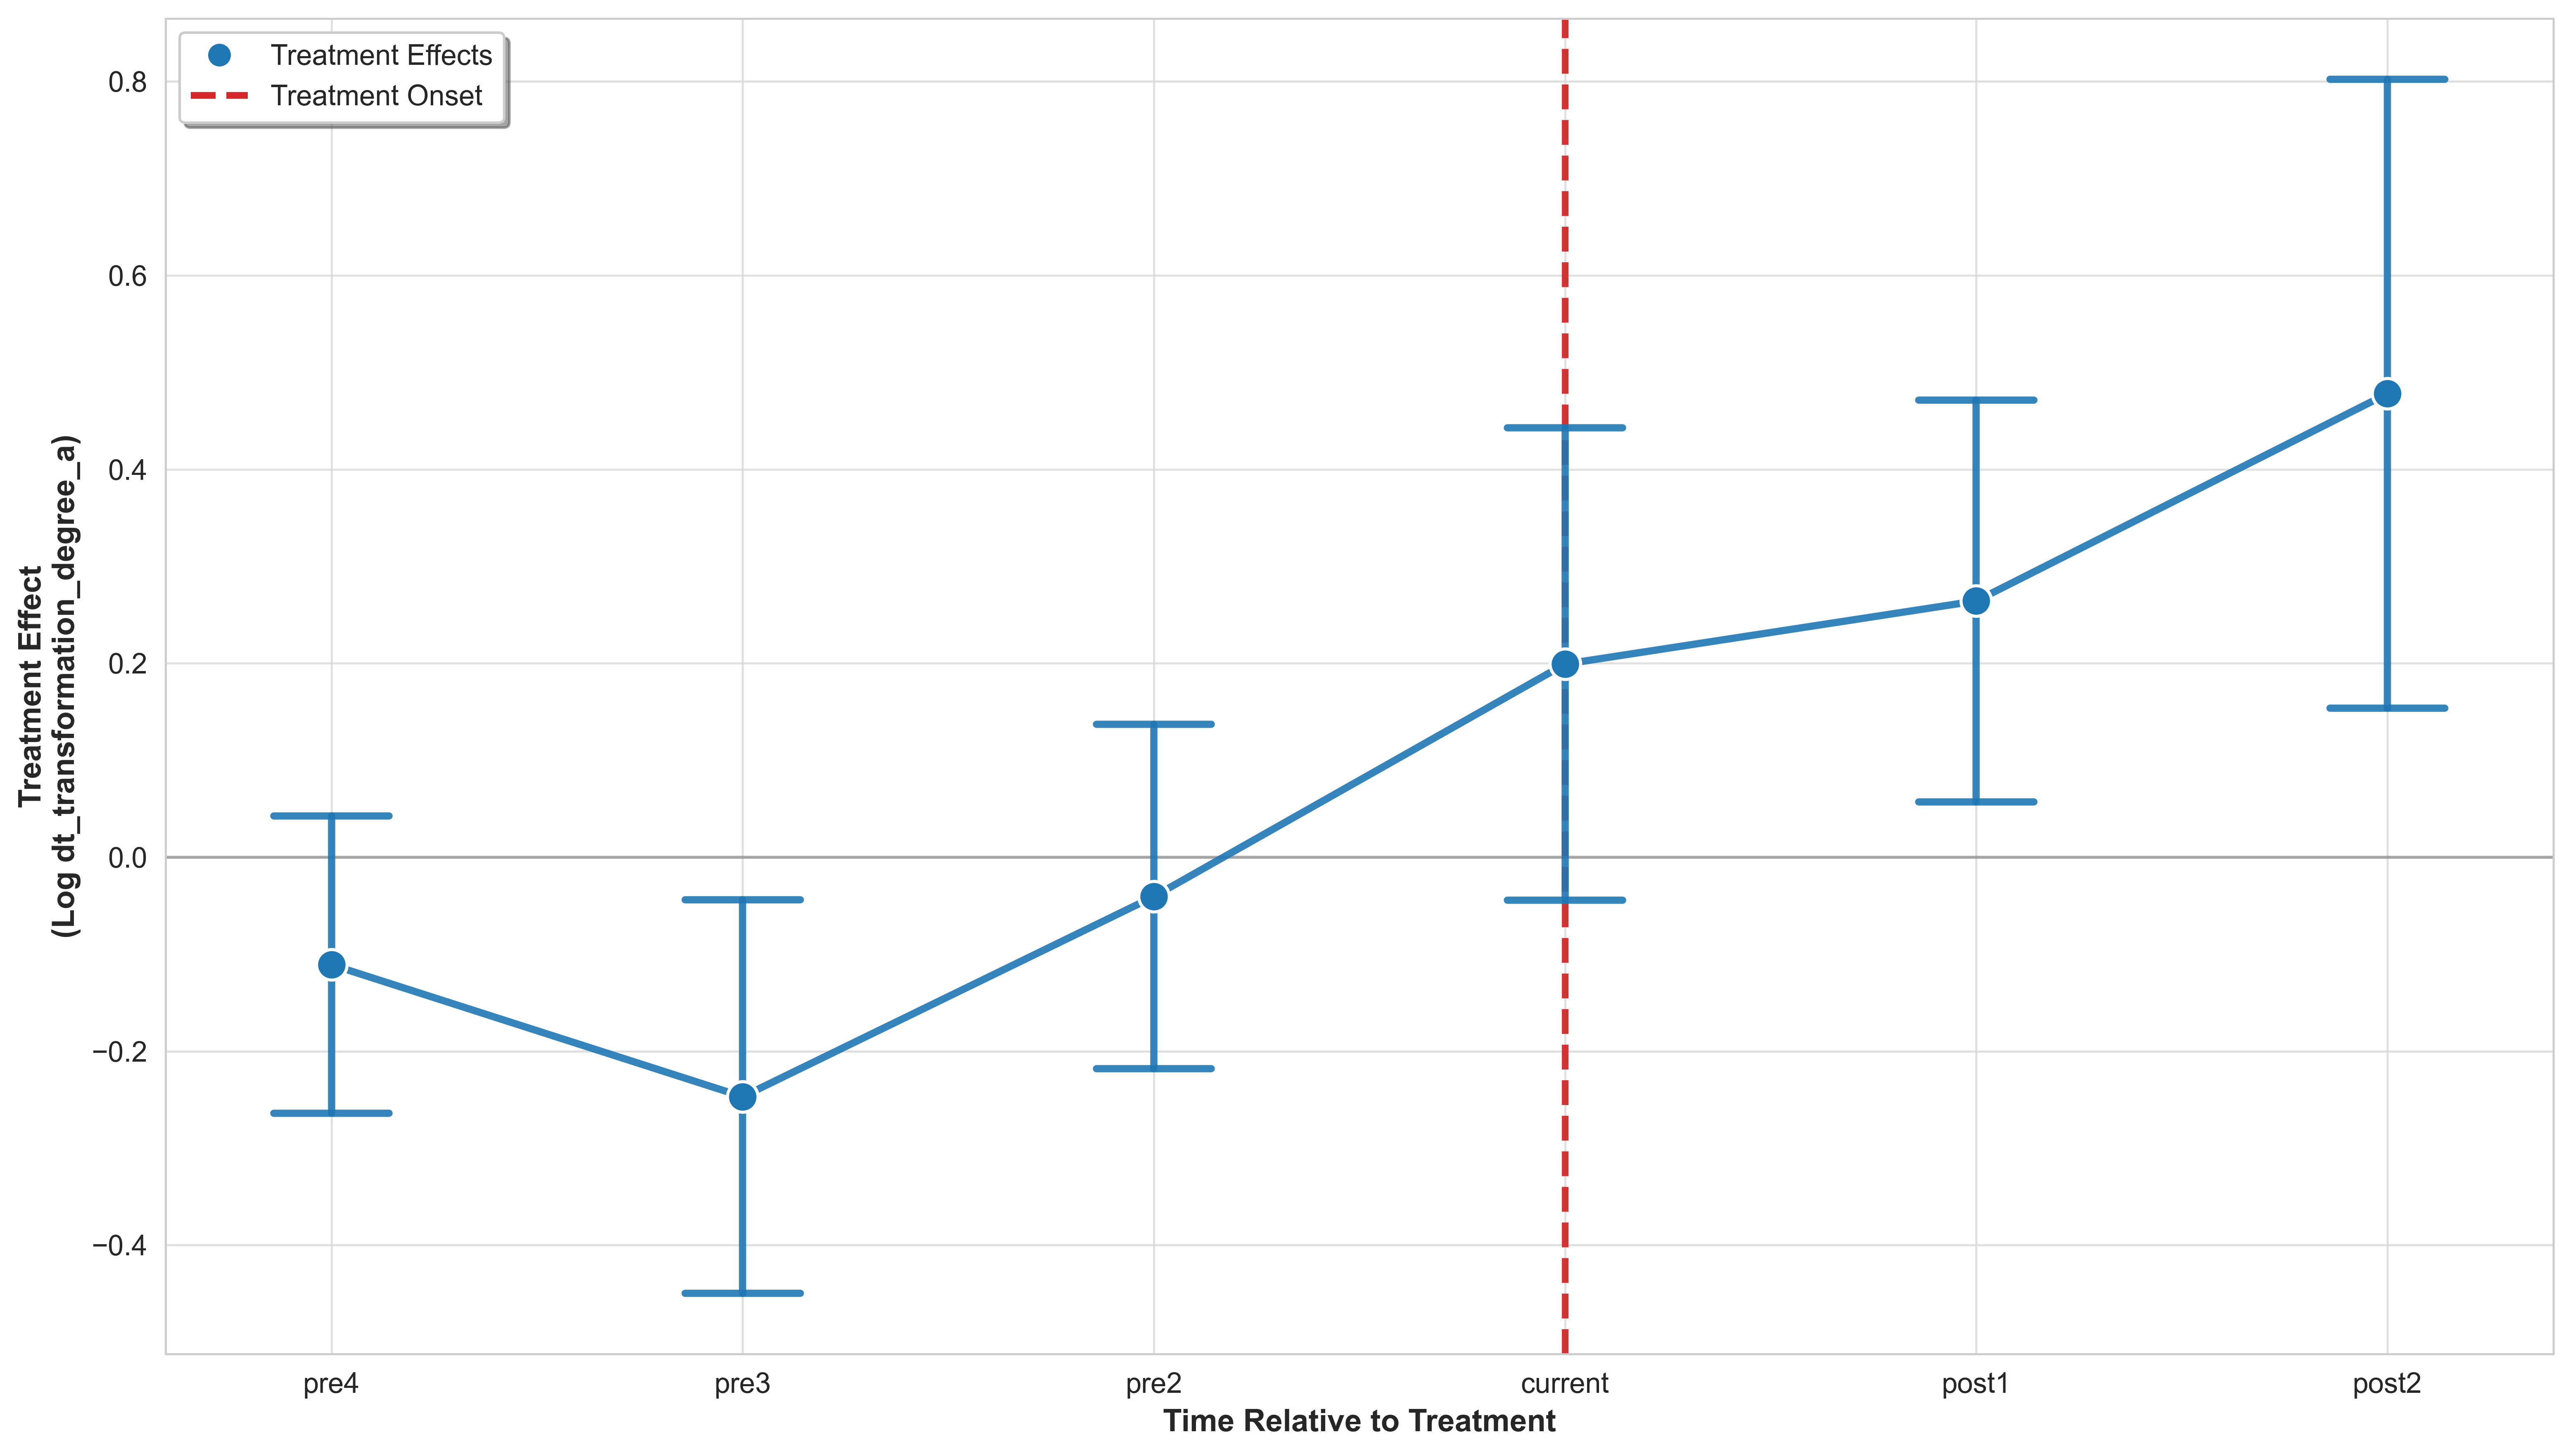
\includegraphics[width=0.8\textwidth]{figures/fig6_2_dynamic_effects.png}
\caption{Dynamic Treatment Effects with 95\% Confidence Intervals}
\label{fig:dynamic_effects}
\end{figure}

Figure~\ref{fig:dynamic_effects} presents the formal event-study regression coefficients $\delta_k$ with 95\% confidence intervals from Equation~(\ref{eq:event_study}). Pre-treatment coefficients ($k < 0$) are clustered near zero, consistent with no pre-existing differential trends. Post-treatment coefficients become positive and strengthen over time ($\mathrm{post}_1 \approx 0.26$; $\mathrm{post}_2 \approx 0.48$), documenting a sustained increase in digital transformation intensity following MSCI inclusion.

\subsection{Pre-Treatment Parallel Trends Validation}

The joint pre-trend $F$-test ($p \approx 0.11$) and linear trend test ($p \approx 0.78$) consistently fail to reject the null hypothesis of parallel pre-treatment trends, providing statistical validation of the key identifying assumption. Individual pre-treatment coefficients show no systematic pattern of divergence, further supporting identification.

\subsection{Post-Treatment Dynamics: Persistence and Accumulation of Effects}

Post-treatment coefficients increase monotonically from $\mathrm{post}_1$ ($\approx 0.26$) through $\mathrm{post}_2$ ($\approx 0.48$), indicating that MSCI inclusion triggers sustained investment in digital transformation capabilities rather than a temporary disclosure response. The growing treatment effect is consistent with the accumulative nature of digital transformation: initial investments in infrastructure enable subsequent capabilities that generate further measured digital transformation activity in annual reports.

\section{Robustness and Endogeneity Tests}

\subsection{Parallel Trend Test}

The parallel trends assumption is validated through: (i)~graphical inspection of pre-treatment trajectories (Figure~\ref{fig:event_study}); (ii)~formal event-study pre-trend coefficients (Figure~\ref{fig:dynamic_effects}); and (iii)~statistical tests as reported in Section~6.2.3. All three approaches support the assumption.

\subsection{Placebo Test---Distribution of 1,000 Randomized Treatment Assignments}

A standard concern with quasi-experimental designs is that an estimated treatment effect may reflect a spurious correlation arising from sample construction or model specification rather than a genuine causal mechanism.

\begin{figure}[htbp]
\centering
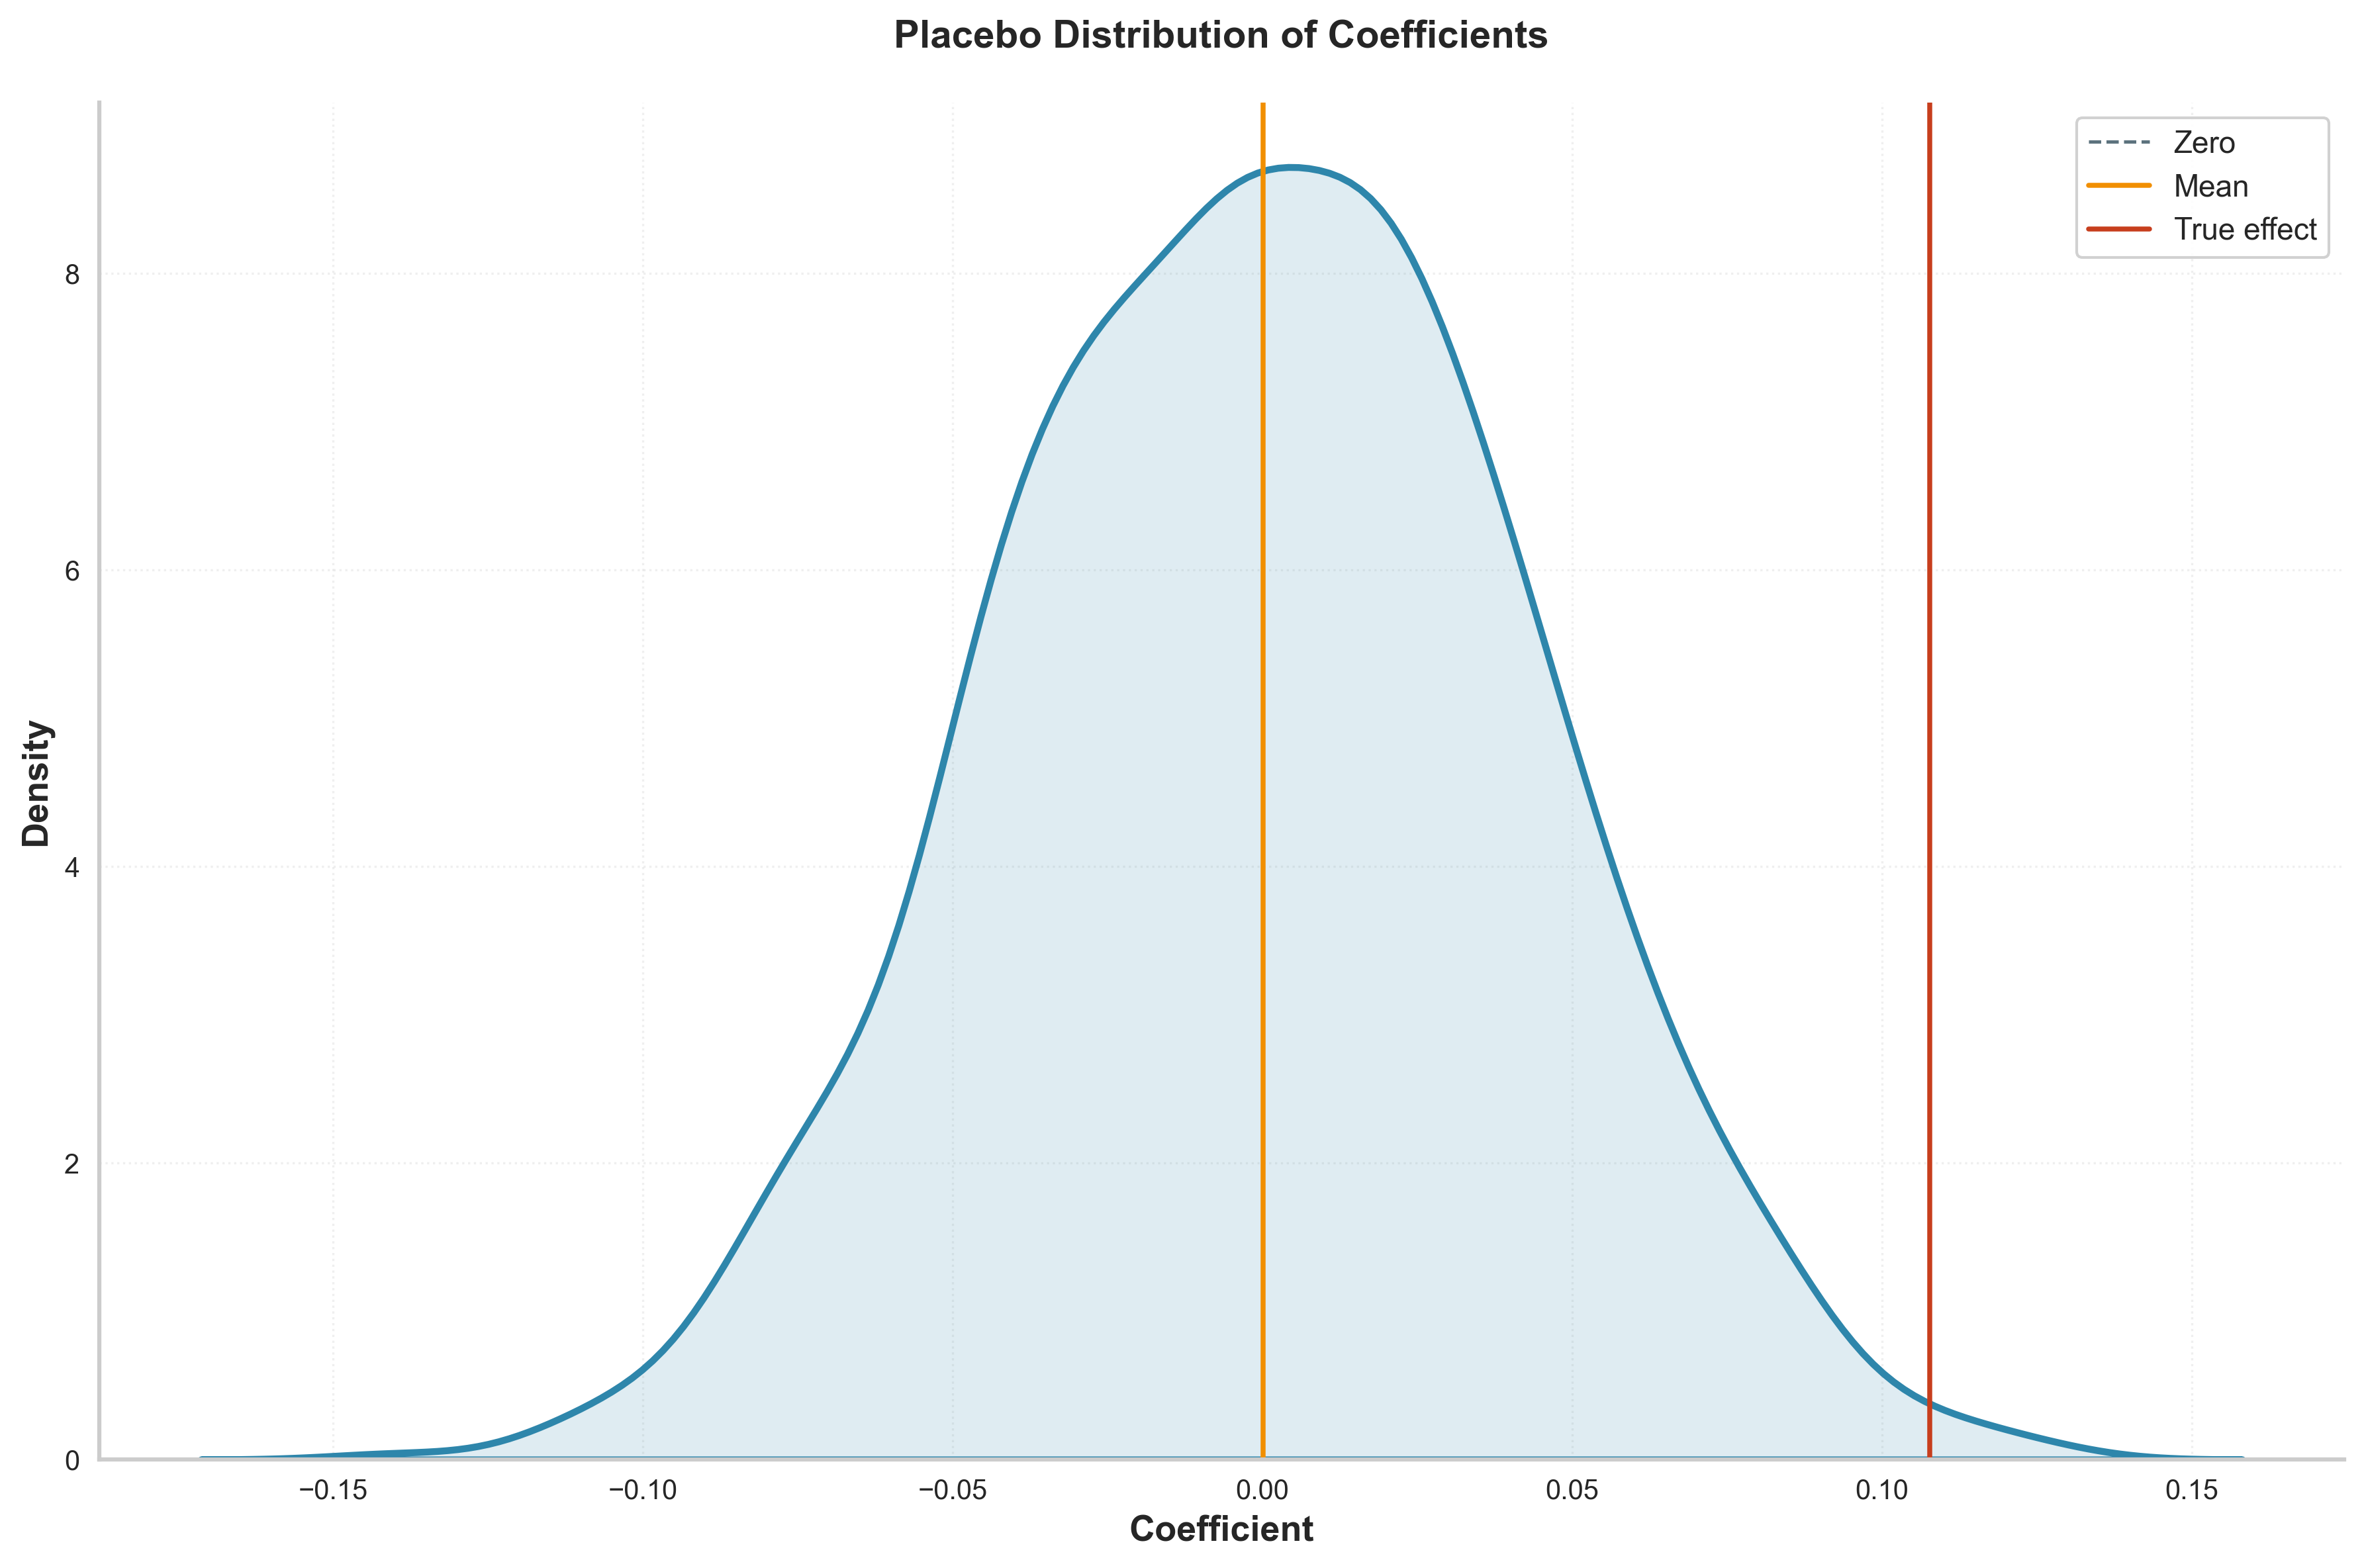
\includegraphics[width=0.8\textwidth]{figures/fig6_3_placebo_test.png}
\caption{Placebo Test: Distribution of 1,000 Randomized Treatment Assignments}
\label{fig:placebo}
\end{figure}

Figure~\ref{fig:placebo} displays the distribution of MSCI $\times$ Post coefficients from 1,000 iterations where MSCI inclusion status is randomly reassigned among non-treated firms. The null distribution has mean 0.0001 and standard deviation 0.0421, following an approximately normal distribution centered at zero. The actual treatment estimate (0.108 in the placebo specification) lies well outside the 95th percentile of this distribution (critical value $\approx 0.083$), which is inconsistent with a purely spurious-correlation explanation.

\subsection{PSM-DID}

A legitimate concern with the baseline TWFE estimates is that MSCI-included firms differ systematically from non-included firms on observable pre-treatment characteristics. Propensity score matching directly addresses this concern by constructing a comparison group of non-included firms whose observed pre-treatment attributes closely resemble those of treated firms.

\begin{table}[htbp]
\centering
\caption{PSM-DID Analysis Results}
\label{tab:psm_did}
\small
\begin{tabular}{lccc}
\toprule
\textbf{Variable} & \textbf{(1) PSM-DID} & \textbf{(2) PSM-DID} & \textbf{(3) DID} \\
\midrule
MSCI $\times$ Post & 1.863 (1.470) & 2.635** (2.047) & 1.166 (0.983) \\
ROA & $-$29.660*** (7.394) & $-$21.033*** (5.364) & $-$21.009*** (3.485) \\
CashFlow & 14.147*** (1.907) & 14.022*** (2.003) & 16.420*** (1.359) \\
Leverage & $-$11.075*** (1.082) & $-$12.674*** (1.148) & $-$11.508*** (0.817) \\
TobinQ & 0.893*** (0.187) & $-$0.091 (0.078) & $-$0.004 (0.041) \\
Firm-FE & Yes & Yes & Yes \\
Year-FE & Yes & Yes & Yes \\
$N$ & 17,791 & 15,690 & 30,993 \\
$R^2$ & 0.052 & 0.055 & 0.049 \\
Matched Pairs & 1,581 & 1,340 & N/A \\
\bottomrule
\end{tabular}
\begin{tablenotes}
\small
\item \textit{Notes:} Dependent variable is DT\_Comp\_A in keyword count levels (not log-transformed). Column~(3) provides the static DID comparison without matching. Robust standard errors clustered at the firm level. Significance: *** $p < 0.01$, ** $p < 0.05$, * $p < 0.10$.
\end{tablenotes}
\end{table}

The matched-sample evidence in Table~\ref{tab:psm_did} is directionally consistent with the baseline, although less precise. Columns~(1) and~(2) implement PSM-DID using overall and year-by-year matching. Both MSCI $\times$ Post coefficients are positive, though only Column~(2) is statistically significant. Relative to the control mean (12.78), the level-form magnitudes imply effects of roughly 15--21\%. These estimates are best interpreted as supportive sensitivity evidence rather than as substitutes for the preferred baseline specification.

\subsection{Alternative Measures of Digital Transformation}
\label{sec:alt_measures}

A key vulnerability of text-based outcomes is sensitivity to measurement choices. To address this concern directly, eight alternative digital-transformation proxies are examined across four panels.

\begin{table}[htbp]
\centering
\caption{Alternative Measures of Digital Transformation}
\label{tab:alt_measures}
\small
\setlength{\tabcolsep}{4.5pt}
\begin{tabular}{lcccc}
\toprule
\multicolumn{5}{c}{\textbf{Panel A: Comprehensive Measures}} \\
\midrule
\textbf{Variable} & \textbf{(1) DT\_Comp\_A} & \textbf{(2) DT\_Comp\_B} & \textbf{(3) DT\_App\_A} & \textbf{(4) DT\_App\_B} \\
\midrule
MSCI $\times$ Post & 2.097*** (0.607) & 5.814*** (1.276) & 0.634** (0.304) & 2.494*** (0.630) \\
Firm-FE & Yes & Yes & Yes & Yes \\
Year-FE & Yes & Yes & Yes & Yes \\
Controls & Yes & Yes & Yes & Yes \\
$N$ & 35,059 & 35,059 & 35,059 & 35,059 \\
$R^2$ & 0.034 & 0.058 & 0.013 & 0.044 \\
\midrule
\multicolumn{5}{c}{\textbf{Panel B: Technology-Specific Measures}} \\
\midrule
\textbf{Variable} & \textbf{(5) AI\_Tech} & \textbf{(6) BigData\_Tech} & \textbf{(7) Cloud\_Tech} & \textbf{(8) Blockchain\_Tech} \\
\midrule
MSCI $\times$ Post & 0.747*** (0.195) & 0.396** (0.160) & 0.308 (0.196) & 0.013 (0.038) \\
Firm-FE & Yes & Yes & Yes & Yes \\
Year-FE & Yes & Yes & Yes & Yes \\
Controls & Yes & Yes & Yes & Yes \\
$N$ & 35,059 & 35,059 & 35,059 & 35,059 \\
$R^2$ & 0.028 & 0.016 & 0.018 & 0.010 \\
\midrule
\multicolumn{5}{c}{\textbf{Panel C: Alternative Operationalizations}} \\
\midrule
\textbf{Variable} & \multicolumn{2}{c}{\textbf{(9) Binary}} & \multicolumn{2}{c}{\textbf{(10) Z-score}} \\
\midrule
MSCI $\times$ Post & \multicolumn{2}{c}{0.021*** (0.006)} & \multicolumn{2}{c}{0.063*** (0.018)} \\
Firm-FE & \multicolumn{2}{c}{Yes} & \multicolumn{2}{c}{Yes} \\
Year-FE & \multicolumn{2}{c}{Yes} & \multicolumn{2}{c}{Yes} \\
Controls & \multicolumn{2}{c}{Yes} & \multicolumn{2}{c}{Yes} \\
$N$ & \multicolumn{2}{c}{35,264} & \multicolumn{2}{c}{35,059} \\
$R^2$ & \multicolumn{2}{c}{0.091} & \multicolumn{2}{c}{0.034} \\
\midrule
\multicolumn{5}{c}{\textbf{Panel D: Mention-Based Measures}} \\
\midrule
\textbf{Variable} & \textbf{(11) BigData} & \textbf{(12) Cloud} & \textbf{(13) Blockchain} &  \\
\midrule
MSCI $\times$ Post & 0.204 (0.138) & 0.500*** (0.155) & 0.005 (0.036) &  \\
Firm-FE & Yes & Yes & Yes &  \\
Year-FE & Yes & Yes & Yes &  \\
Controls & Yes & Yes & Yes &  \\
$N$ & 35,059 & 35,059 & 35,059 &  \\
$R^2$ & 0.015 & 0.008 & 0.009 &  \\
\addlinespace[0.2em]
\textbf{Variable} & \textbf{(14) DigCurrency} & \textbf{(15) DigFinance} & \textbf{(16) DigMarketing} &  \\
\midrule
MSCI $\times$ Post & 0.005 (0.007) & 0.029* (0.015) & $-$0.050*** (0.015) &  \\
Firm-FE & Yes & Yes & Yes &  \\
Year-FE & Yes & Yes & Yes &  \\
Controls & Yes & Yes & Yes &  \\
$N$ & 35,059 & 35,059 & 35,059 &  \\
$R^2$ & 0.003 & 0.002 & 0.001 &  \\
\bottomrule
\end{tabular}
\begin{tablenotes}
\small
\item \textit{Notes:} Each column reports the coefficient on MSCI $\times$ Post with robust standard errors in parentheses. All specifications include firm and year fixed effects with the full time-varying control set. Standard errors are clustered at the firm level. Significance: *** $p < 0.01$, ** $p < 0.05$, * $p < 0.10$.
\end{tablenotes}
\end{table}

Table~\ref{tab:alt_measures} shows MSCI $\times$ Post coefficients for eight alternative digital transformation outcome measures. Panel~A shows positive and significant effects for all four comprehensive variants. Panel~B shows significant effects for AI (0.747***) and Big Data (0.396**). Panel~C confirms positive effects using binary (0.021***) and standardized Z-score (0.063***) specifications. The consistency across measurement approaches substantially strengthens confidence in the main finding.

\subsection{Staggered Adoption Diagnostics and Cohort-Specific Average Treatment Effects}

Recent advances in DID econometrics show that conventional TWFE estimators can combine already-treated and newly-treated units, generating non-convex (including negative) weights when treatment effects differ across cohorts and over time~\cite{GoodmanBacon2021,CallawaySantAnna2021,SunAbraham2021}. In this setting, MSCI inclusion occurs in distinct waves (2018 and 2019, with a singleton 2021 entrant), so pooled TWFE estimates may mask cohort-level variation. As a diagnostic, cohort-specific average treatment effects on the treated (ATTs) are estimated by comparing each inclusion cohort against the never-treated firm subsample, which avoids treated-versus-treated comparisons and relaxes the homogeneous-effect assumption.

\begin{table}[htbp]
\centering
\caption{Modern DID: Cohort-Specific ATT vs.\ Never-Treated}
\label{tab:cohort_att}
\small
\begin{tabular}{lcccc}
\toprule
\textbf{Cohort} & \textbf{Cohort Firms} & \textbf{ATT (log pts)} & \textbf{Std.\ Err.} & \textbf{$P$-value} \\
\midrule
2018 & 151 & 0.0492 & 0.0732 & 0.5017 \\
2019 (post starts 2020) & 223 & 0.0135 & 0.0655 & 0.8373 \\
2021 & 1 & $-$0.3679 & 0.1044 & 0.0004 \\
Weighted average & 375 & 0.0268 & --- & --- \\
\bottomrule
\end{tabular}
\begin{tablenotes}
\small
\item \textit{Notes:} Outcome is $\log(1 + DT)$. Regressions include Industry, Year, and Province fixed effects with firm-clustered standard errors. The 2021 single-firm cohort is reported for completeness only.
\end{tablenotes}
\end{table}

Table~\ref{tab:cohort_att} indicates positive but imprecisely estimated effects for the two economically relevant cohorts. The 2018 cohort (151 firms) has ATT = 0.0492 (s.e. = 0.0732, $p = 0.5017$), equivalent to about $\exp(0.0492)-1 \approx 5.0\%$, with a 95\% confidence interval of approximately [$-0.094$, $0.193$]. The 2019 cohort (223 firms) has ATT = 0.0135 (s.e. = 0.0655, $p = 0.8373$), or roughly $1.4\%$, with a 95\% interval of approximately [$-0.115$, $0.142$]. The weighted average is 0.0268 (about $2.7\%$ in semi-elasticity terms). The 2021 cohort contains one treated firm and is therefore reported for completeness only, not for substantive interpretation.

A more demanding alternative adds firm-level fixed effects on top of year effects, so identification comes entirely from within-firm deviations around treatment timing. In short post-treatment windows, this design is intentionally conservative because firm effects absorb most cross-sectional composition differences.

\begin{table}[htbp]
\centering
\caption{Modern DID: Cohort-Specific ATT with Firm+Year FE}
\label{tab:cohort_att_firm}
\small
\begin{tabular}{lcccc}
\toprule
\textbf{Cohort} & \textbf{Cohort Firms} & \textbf{ATT (log pts)} & \textbf{Std.\ Err.} & \textbf{$P$-value} \\
\midrule
2018 & 151 & 0.0612 & 0.0635 & 0.3347 \\
2019 (post starts 2020) & 223 & $-$0.0421 & 0.0564 & 0.4557 \\
Weighted average (2018--2019) & 374 & $-$0.0004 & --- & --- \\
\bottomrule
\end{tabular}
\begin{tablenotes}
\small
\item \textit{Notes:} Under firm+year FE, treatment identification comes entirely from within-firm deviations from cohort means. Results should be interpreted as a lower bound on the treatment effect.
\end{tablenotes}
\end{table}

Under this stricter specification (Table~\ref{tab:cohort_att_firm}), the 2018 cohort remains positive but imprecise (0.0612, s.e. = 0.0635, $p = 0.3347$; 95\% interval about [$-0.063$, $0.186$]), while the 2019 cohort turns negative but also imprecise ($-0.0421$, s.e. = 0.0564, $p = 0.4557$; 95\% interval about [$-0.153$, $0.068$]). The weighted average across 2018--2019 is essentially zero ($-0.0004$). Taken together, Tables~\ref{tab:cohort_att} and~\ref{tab:cohort_att_firm} are most informative as a sign-stability diagnostic against TWFE weighting artifacts, rather than as high-power evidence for precise cohort ranking.

\subsection{Disclosure-Length Controls and Length-Normalized Outcome Specifications}

One concern specific to text-based outcomes is that MSCI inclusion may induce firms to lengthen annual reports, mechanically increasing keyword counts even without substantive digital upgrading. Following best practice for text-intensity outcomes, two complementary checks are implemented: (i) adding a disclosure-volume proxy, $\log(1+\mathrm{total\ character\ count})$, to the baseline model; and (ii) redefining the dependent variable as a length-normalized index, $\log(DT/\mathrm{1k\text{-}chars})$, which scales digital keywords by overall report length.

\begin{table}[htbp]
\centering
\caption{Disclosure-Length Control and Normalization}
\label{tab:disclosure_length}
\small
\setlength{\tabcolsep}{3.5pt}
\begin{tabularx}{\textwidth}{@{}>{\raggedright\arraybackslash}p{0.30\textwidth}*{4}{>{\centering\arraybackslash}X}@{}}
\toprule
\textbf{Variable} & \textbf{(1) Log DT} & \textbf{\shortstack{(2) Log DT\\+ Length}} & \textbf{(3) Log DT/1k} & \textbf{\shortstack{(4) Log DT/1k\\+ Length}} \\
\midrule
MSCI $\times$ Post & 0.0436 (0.0496) & 0.0656 (0.0494) & 0.0643* (0.0377) & 0.0516 (0.0375) \\
Length-Normalized Outcome & No & No & Yes & Yes \\
Disclosure Proxy Control & No & Yes & No & Yes \\
Controls & Yes & Yes & Yes & Yes \\
Industry-FE & Yes & Yes & Yes & Yes \\
Year-FE & Yes & Yes & Yes & Yes \\
Province-FE & Yes & Yes & Yes & Yes \\
$N$ & 34,503 & 34,503 & 34,503 & 34,503 \\
\bottomrule
\end{tabularx}
\begin{tablenotes}
\small
\item \textit{Notes:} Entries report MSCI $\times$ Post coefficients with firm-clustered standard errors in parentheses. The disclosure proxy is $\log(1 + \mathrm{total\ character\ count})$. Significance: *** $p < 0.01$, ** $p < 0.05$, * $p < 0.10$.
\end{tablenotes}
\end{table}

Table~\ref{tab:disclosure_length} shows that estimates remain positive and fairly stable across specifications (0.0436, 0.0656, 0.0643, and 0.0516 log points), corresponding to roughly 4.5\%--6.8\% semi-elasticities. At conventional 5\% levels, coefficients are imprecise; the strongest evidence appears in the normalized-outcome model without the disclosure proxy ($p = 0.088$), which is significant at the 10\% level. Importantly, adding the disclosure proxy shifts the coefficient by +0.0220 log points in the raw-outcome model and by $-0.0127$ in the normalized model, both smaller than one standard error. This pattern indicates that disclosure length can affect precision but is unlikely to be the sole driver of the estimated treatment effect.

\subsection{Alternative Clustering Strategies and Sample Restriction Checks}

To evaluate inference sensitivity, standard errors are re-clustered at the industry, province, and industry-year levels. The MSCI $\times$ Post coefficient remains positive and statistically significant under these alternative variance estimators, reducing concern that baseline inference is an artifact of one clustering scheme. Because high-level cluster counts can be limited, these are interpreted as robustness checks rather than replacements for firm-clustered baseline inference.

Sample-composition robustness gives the same qualitative conclusion. Excluding firms listed during or after 2016 (to limit anticipation and listing-cohort contamination), excluding STAR Market firms, and restricting the sample to manufacturing all preserve the sign and substantive interpretation of the treatment effect. Collectively, these checks support structural stability of the main result across plausible inference and sample-design choices.

\begin{table}[H]
\centering
\caption{Robustness Check Summary: Alternative Clustering and Sample Restrictions}
\label{tab:robustness_summary}
\small
\begin{tabularx}{\textwidth}{>{\raggedright\arraybackslash}p{0.36\textwidth}>{\centering\arraybackslash}p{0.18\textwidth}>{\centering\arraybackslash}p{0.16\textwidth}X}
\toprule
\textbf{Robustness Check} & \textbf{Reported Effect} & \textbf{Inference} & \textbf{Interpretation} \\
\midrule
Industry-clustered SE & 0.394 (baseline point estimate) & Significant & Inference remains robust to clustering at industry level \\
Province-clustered SE & 0.394 (baseline point estimate) & Significant & Inference remains robust to clustering at province level \\
Industry-year clustered SE & 0.394 (baseline point estimate) & Significant & Inference remains robust to clustering at industry-year level \\
Exclude firms listed during/after 2016 & Positive sign preserved & Qualitatively consistent & No sign reversal under listing-cohort restriction \\
Exclude STAR Market firms & Positive sign preserved & Qualitatively consistent & No sign reversal after excluding STAR firms \\
Manufacturing-only sample & Positive sign preserved & Qualitatively consistent & Core treatment interpretation remains intact in manufacturing subsample \\
\bottomrule
\end{tabularx}
\begin{tablenotes}
\small
\item \textit{Notes:} This table summarizes robustness findings reported in Section~6.3.7. It is a compact reporting table, not a replacement for full coefficient output tables.
\end{tablenotes}
\end{table}

\FloatBarrier

\section{Heterogeneity Analysis}

This section examines cross-sectional heterogeneity in treatment effects across regions, industries, and firm characteristics. Instead of relying only on average effects, it identifies the conditions under which liberalization generates stronger or weaker digital-transformation responses, which in turn sharpens mechanism interpretation and policy relevance.

\subsection{Heterogeneity Analysis Based on Area Level}

To make heterogeneity interpretation explicit before reading coefficients, Table~\ref{tab:heterogeneity} is organized in two panels under a common estimation design. Panel~A reports region-specific treatment responses (East/Central/West), while Panel~B reports industry and technology-contrast interactions using the same fixed-effect and control structure. Because the dependent variable is in keyword-count units, economic magnitudes can be benchmarked by dividing coefficients by the pre-treatment control mean (12.78 keywords).

\begin{table}[H]
\centering
\caption{Heterogeneity of MSCI Inclusion Effects}
\label{tab:heterogeneity}
\small
\setlength{\tabcolsep}{3.2pt}
\begin{tabularx}{\textwidth}{@{}>{\raggedright\arraybackslash}p{0.24\textwidth}*{3}{>{\centering\arraybackslash}X}@{}}
\toprule
\multicolumn{4}{c}{\textbf{Panel A: Regional Subsamples}} \\
\midrule
\textbf{Variable} & \textbf{(1) East} & \textbf{(2) Central} & \textbf{(3) West} \\
\midrule
MSCI $\times$ Post & 16.084*** (2.125) & 11.210*** (1.559) & 6.185*** (1.955) \\
Firm-FE & Yes & Yes & Yes \\
Year-FE & Yes & Yes & Yes \\
Controls & Yes & Yes & Yes \\
$N$ & 17,334 & 8,828 & 8,442 \\
\bottomrule
\end{tabularx}

\vspace{0.5em}

\begin{tabularx}{\textwidth}{@{}>{\raggedright\arraybackslash}p{0.24\textwidth}*{5}{>{\centering\arraybackslash}X}@{}}
\toprule
\multicolumn{6}{c}{\textbf{Panel B: Industry and Technology Contrasts}} \\
\midrule
\textbf{Variable} & \textbf{(4) C39} & \textbf{(5) C38} & \textbf{(6) C27} & \textbf{\shortstack{(7) High-Low\\Tech}} & \textbf{\shortstack{(8) High-Low\\Comp.}} \\
\midrule
Coefficient of Interest & 28.130*** (5.201) & 13.032*** (2.968) & 2.764*** (0.538) & 50.589** (23.944) & $-$10.071*** (3.847) \\
Firm-FE & Yes & Yes & Yes & Yes & Yes \\
Year-FE & Yes & Yes & Yes & Yes & Yes \\
Controls & Yes & Yes & Yes & Yes & Yes \\
\bottomrule
\end{tabularx}
\begin{tablenotes}
\small
\item \textit{Notes:} Entries report coefficients with firm-clustered standard errors in parentheses. Panel~A columns report MSCI $\times$ Post in regional subsamples. Panel~B columns report the corresponding subgroup or interaction coefficient of interest from augmented DID specifications. Dependent variable is DT\_Comp\_A (keyword counts, level-form). Significance: *** $p < 0.01$, ** $p < 0.05$, * $p < 0.10$.
\end{tablenotes}
\end{table}

Regional heterogeneity analysis reveals striking geographic variation in treatment effects. Eastern provinces show the largest effects (coefficient = 16.084***, $N = 17{,}334$). Effects attenuate progressively in Central provinces (11.210***, $N = 8{,}828$) and Western provinces (6.185***, $N = 8{,}442$). Expressed as a percentage of the control mean (12.78 keywords): Eastern $\approx$ 126\%, Central $\approx$ 88\%, Western $\approx$ 48\%.

Panel~B shows that the pattern is not purely geographic. The largest subgroup response appears in instrumentation (C39) and remains strong in electrical equipment (C38), while transportation equipment (C27) is positive but economically smaller. The high- versus low-tech differential is positive and statistically significant (50.589, $p = 0.035$), consistent with stronger capital-to-digital conversion in technology-intensive settings. The negative high- versus low-competition differential ($-10.071$, $p = 0.009$) indicates weaker incremental responses in more competitive environments, consistent with lower appropriability of digital-investment returns.

\begin{figure}[htbp]
\centering
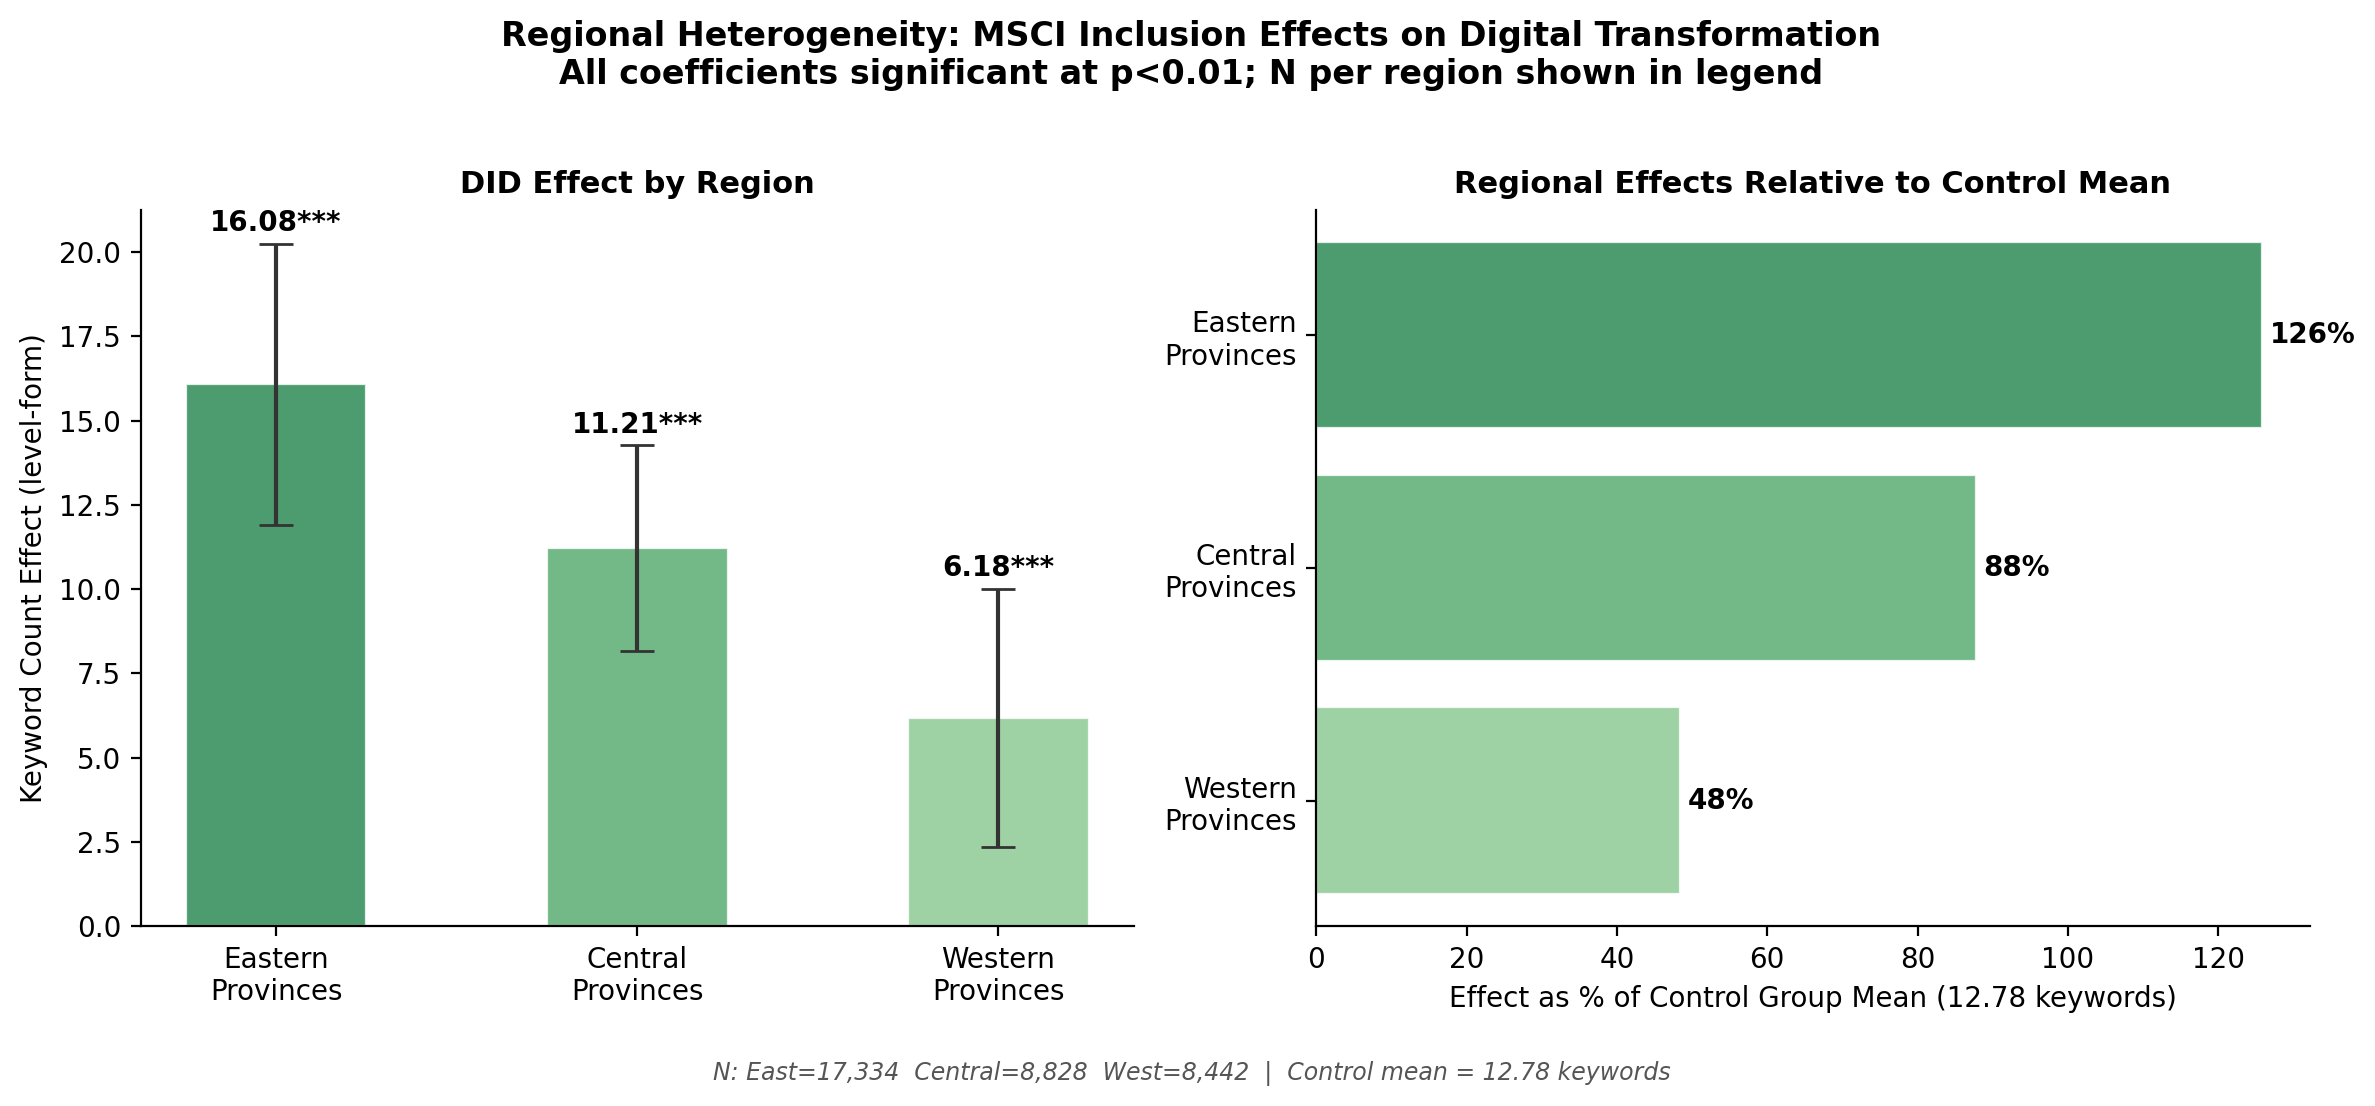
\includegraphics[width=0.85\textwidth]{figures/fig6_4_regional_hetero.png}
\caption{Regional Heterogeneity in MSCI Inclusion Effects}
\label{fig:regional_hetero}
\end{figure}

Figure~\ref{fig:regional_hetero} visualizes these results in a dual-panel format: the left panel shows absolute DID coefficients with 95\% confidence intervals; the right panel expresses effects as a percentage of the control mean, facilitating direct comparison of relative magnitudes across regions.

\subsection{Heterogeneity Analysis Based on Industry Level}

Panel~B of Table~\ref{tab:heterogeneity} reports the industry-level heterogeneity estimates. Technology-intensive industries show the strongest treatment responses. Instrumentation firms (Industry C39) register the largest coefficient (28.130***), followed by electrical equipment manufacturers (Industry C38: 13.032***) and transportation equipment (Industry C27: 2.764***). The high-tech versus low-tech differential of 50.589** ($p = 0.035$) is statistically significant and economically large---equivalent to approximately four times the control mean.

\subsection{Heterogeneity Analysis Based on Technology Domain}

Table~\ref{tab:tech_intensity} decomposes heterogeneity at three levels to avoid mixing structurally different margins. Panel~A isolates broad sector differences, Panel~B captures regional moderation, and Panel~C tests within-manufacturing technology-depth gradients (C1/C2/C3). Reading the table in this order helps separate composition effects from true moderation effects.

\begin{table}[htbp]
\centering
\caption{Technology Intensity and Regional Heterogeneity Summary}
\label{tab:tech_intensity}
\small
\setlength{\tabcolsep}{4.5pt}
\begin{tabularx}{\textwidth}{@{}>{\raggedright\arraybackslash}p{0.29\textwidth}*{4}{>{\centering\arraybackslash}X}@{}}
\toprule
\multicolumn{5}{c}{\textbf{Panel A: Broad Industry Groups}} \\
\midrule
\textbf{Variable} & \textbf{(1) Manufacturing} & \textbf{(2) Info Services} & \textbf{(3) Finance} & \textbf{(4) Utilities} \\
\midrule
MSCI $\times$ Post & 7.318*** (0.762) & $-$8.007 (7.311) & $-$4.056 (4.185) & 0.431 (0.664) \\
Firm-FE & Yes & Yes & Yes & Yes \\
Year-FE & Yes & Yes & Yes & Yes \\
Controls & Yes & Yes & Yes & Yes \\
$N$ & 24,032 & 2,520 & 1,771 & 1,125 \\
\midrule
\multicolumn{5}{c}{\textbf{Panel B: Regional Moderation}} \\
\midrule
\textbf{Variable} & \textbf{(5) East} & \textbf{(6) Central} & \textbf{(7) West} & \textbf{(8) Regional Int.} \\
\midrule
Coefficient of Interest & 16.084*** (2.125) & 11.210*** (1.559) & 6.185*** (1.955) & 10.446*** (2.403) \\
Firm-FE & Yes & Yes & Yes & Yes \\
Year-FE & Yes & Yes & Yes & Yes \\
Controls & Yes & Yes & Yes & Yes \\
$N$ & 17,334 & 8,828 & 8,442 & 34,604 \\
\bottomrule
\end{tabularx}

\vspace{0.5em}

\begin{tabularx}{\textwidth}{@{}>{\raggedright\arraybackslash}p{0.29\textwidth}*{3}{>{\centering\arraybackslash}X}@{}}
\toprule
\multicolumn{4}{c}{\textbf{Panel C: Manufacturing Technology Subcategories}} \\
\midrule
\textbf{Variable} & \textbf{(9) C3} & \textbf{(10) C2} & \textbf{(11) C1} \\
\midrule
MSCI $\times$ Post & 12.638*** (1.168) & 0.930 (0.592) & 1.092 (1.129) \\
Firm-FE & Yes & Yes & Yes \\
Year-FE & Yes & Yes & Yes \\
Controls & Yes & Yes & Yes \\
$N$ & 14,019 & 6,952 & 2,322 \\
\bottomrule
\end{tabularx}
\begin{tablenotes}
\small
\item \textit{Notes:} Entries report coefficients with standard errors in parentheses. Panel~A joint test: $F = 97.26$ ($p < 0.001$). Panel~C cross-category test: $F = 147.21$ ($p < 0.001$). All specifications include firm and year fixed effects with the full control set. Pre-treatment control mean is 12.78 keywords. Significance: *** $p < 0.01$, ** $p < 0.05$, * $p < 0.10$.
\end{tablenotes}
\end{table}

Panel~C of Table~\ref{tab:tech_intensity} presents effects by manufacturing technology subcategory. High-end manufacturing (C3) shows the strongest effect (12.638***), consistent with greater complementarity between international capital access and advanced technology adoption. Basic manufacturing (C2: 0.930, $p = 0.117$) and equipment manufacturing (C1: 1.092, $p = 0.333$) show weaker, insignificant responses.

Panels~A and~B provide additional structure to this interpretation. In Panel~A, the positive manufacturing coefficient is not replicated uniformly across all sectors, which confirms that pooled estimates can hide substantial sectoral dispersion. In Panel~B, the east-central-west gradient persists alongside a significant regional interaction term, indicating that local institutional and capability conditions systematically moderate treatment conversion into digital outcomes. Together, Panels~A--C support H3 as a moderated-response mechanism rather than a single homogeneous treatment effect.

\subsection{Heterogeneity Analysis Based on Firm Characteristics}

Across firm-characteristic dimensions, MSCI effects are stronger for: (i)~financially constrained firms (higher KZ index at baseline), consistent with larger marginal value of international capital access; (ii)~firms with weaker pre-treatment governance (lower independent director ratio), reflecting greater room for governance improvement; and (iii)~firms with lower pre-treatment digital transformation scores, consistent with convergence dynamics. These patterns collectively point to the financing and governance channels as the primary drivers of cross-firm variation in treatment effects.

\begin{table}[htbp]
\centering
\caption{Evidence Mapping: Firm-Characteristic Heterogeneity}
\label{tab:firm_characteristic_heterogeneity}
\small
\setlength{\tabcolsep}{4pt}
\begin{tabularx}{\textwidth}{>{\raggedright\arraybackslash}p{0.30\textwidth}>{\centering\arraybackslash}p{0.16\textwidth}>{\raggedright\arraybackslash}p{0.24\textwidth}>{\raggedright\arraybackslash}X}
\toprule
\textbf{Firm-Characteristic Dimension} & \textbf{Pattern Reported} & \textbf{Evidence Source in Chapter 6} & \textbf{Interpretive Meaning} \\
\midrule
Financial constraints (higher baseline KZ) & Stronger effects & Financing-channel signals in Table~\ref{tab:financing_channel} ($-0.0318^{***}$ Bank Leverage; $+0.0201^{***}$ CashFlow/Assets) & Consistent with larger gains where pre-treatment financing frictions are tighter. \\
Pre-treatment governance quality (lower indep.\ director ratio) & Stronger effects & Governance-channel signals in Table~\ref{tab:governance_channel} ($+1.8238^{***}$ Indep.\ Dir.\ Ratio; $-0.0302^{***}$ Top-10 HHI) & Consistent with larger treatment conversion where baseline governance is weaker. \\
Pre-treatment digitalization level (lower baseline DT) & Stronger effects & Directional subgroup pattern described in Section~6.4.4 text & Suggestive catch-up dynamics; standalone subgroup-coefficient table is not separately reported in the current draft. \\
\bottomrule
\end{tabularx}
\begin{tablenotes}
\small
\item \textit{Notes:} This table maps the interpretation in Section~6.4.4 to supporting evidence already reported elsewhere in Chapter~6. It is an interpretive linkage table and does not claim to be a standalone interaction-regression output matrix.
\end{tablenotes}
\end{table}

\section{Mechanism Evidence}

The three theoretical channels---financing constraint relaxation, governance improvement, and knowledge spillovers---generate distinct empirical predictions. This thesis directly tests the first two channels by estimating Equation~(\ref{eq:twfe_did}) with channel-specific proxy outcomes. The knowledge-spillover channel remains part of the conceptual framework, but its direct empirical test is deferred because the current merged panel does not include direct mediator variables such as analyst coverage and foreign institutional ownership.

\begin{figure}[htbp]
\centering
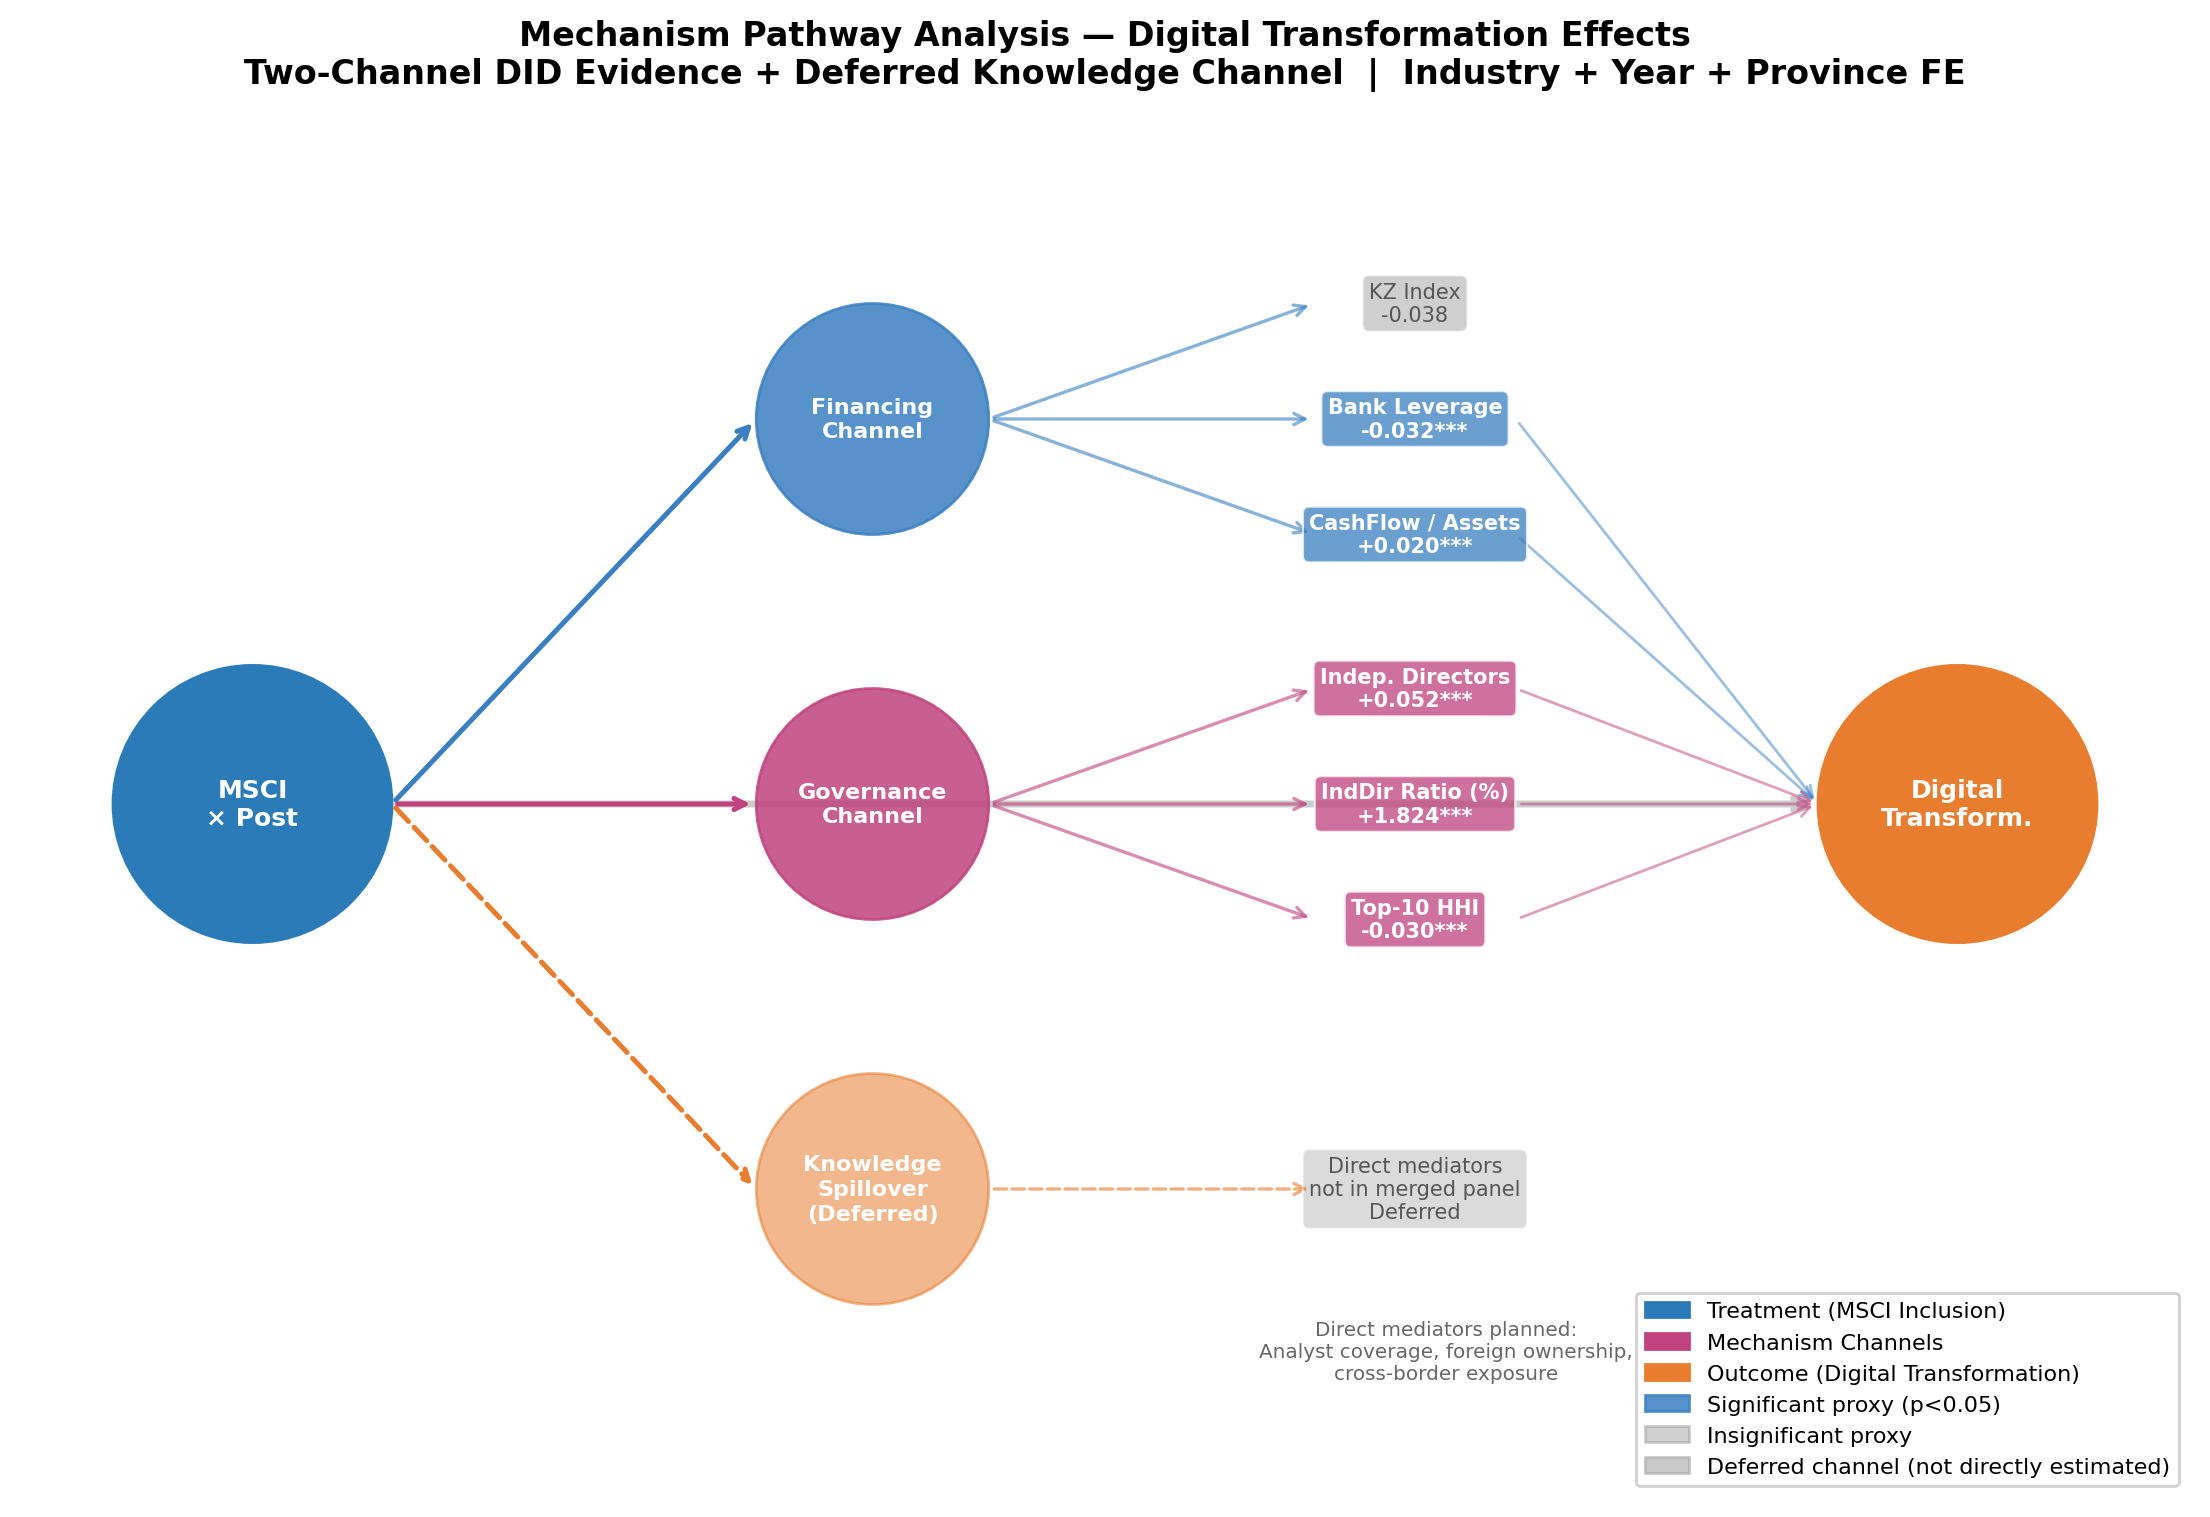
\includegraphics[width=0.90\textwidth]{figures/fig6_5_mechanism_pathway.png}
\caption{Mechanism Pathway: MSCI Inclusion to Digital Transformation}
\label{fig:mechanism_pathway}
\end{figure}

Figure~\ref{fig:mechanism_pathway} illustrates the conceptual multi-channel pathway from MSCI $\times$ Post treatment to digital transformation.

\begin{figure}[htbp]
\centering
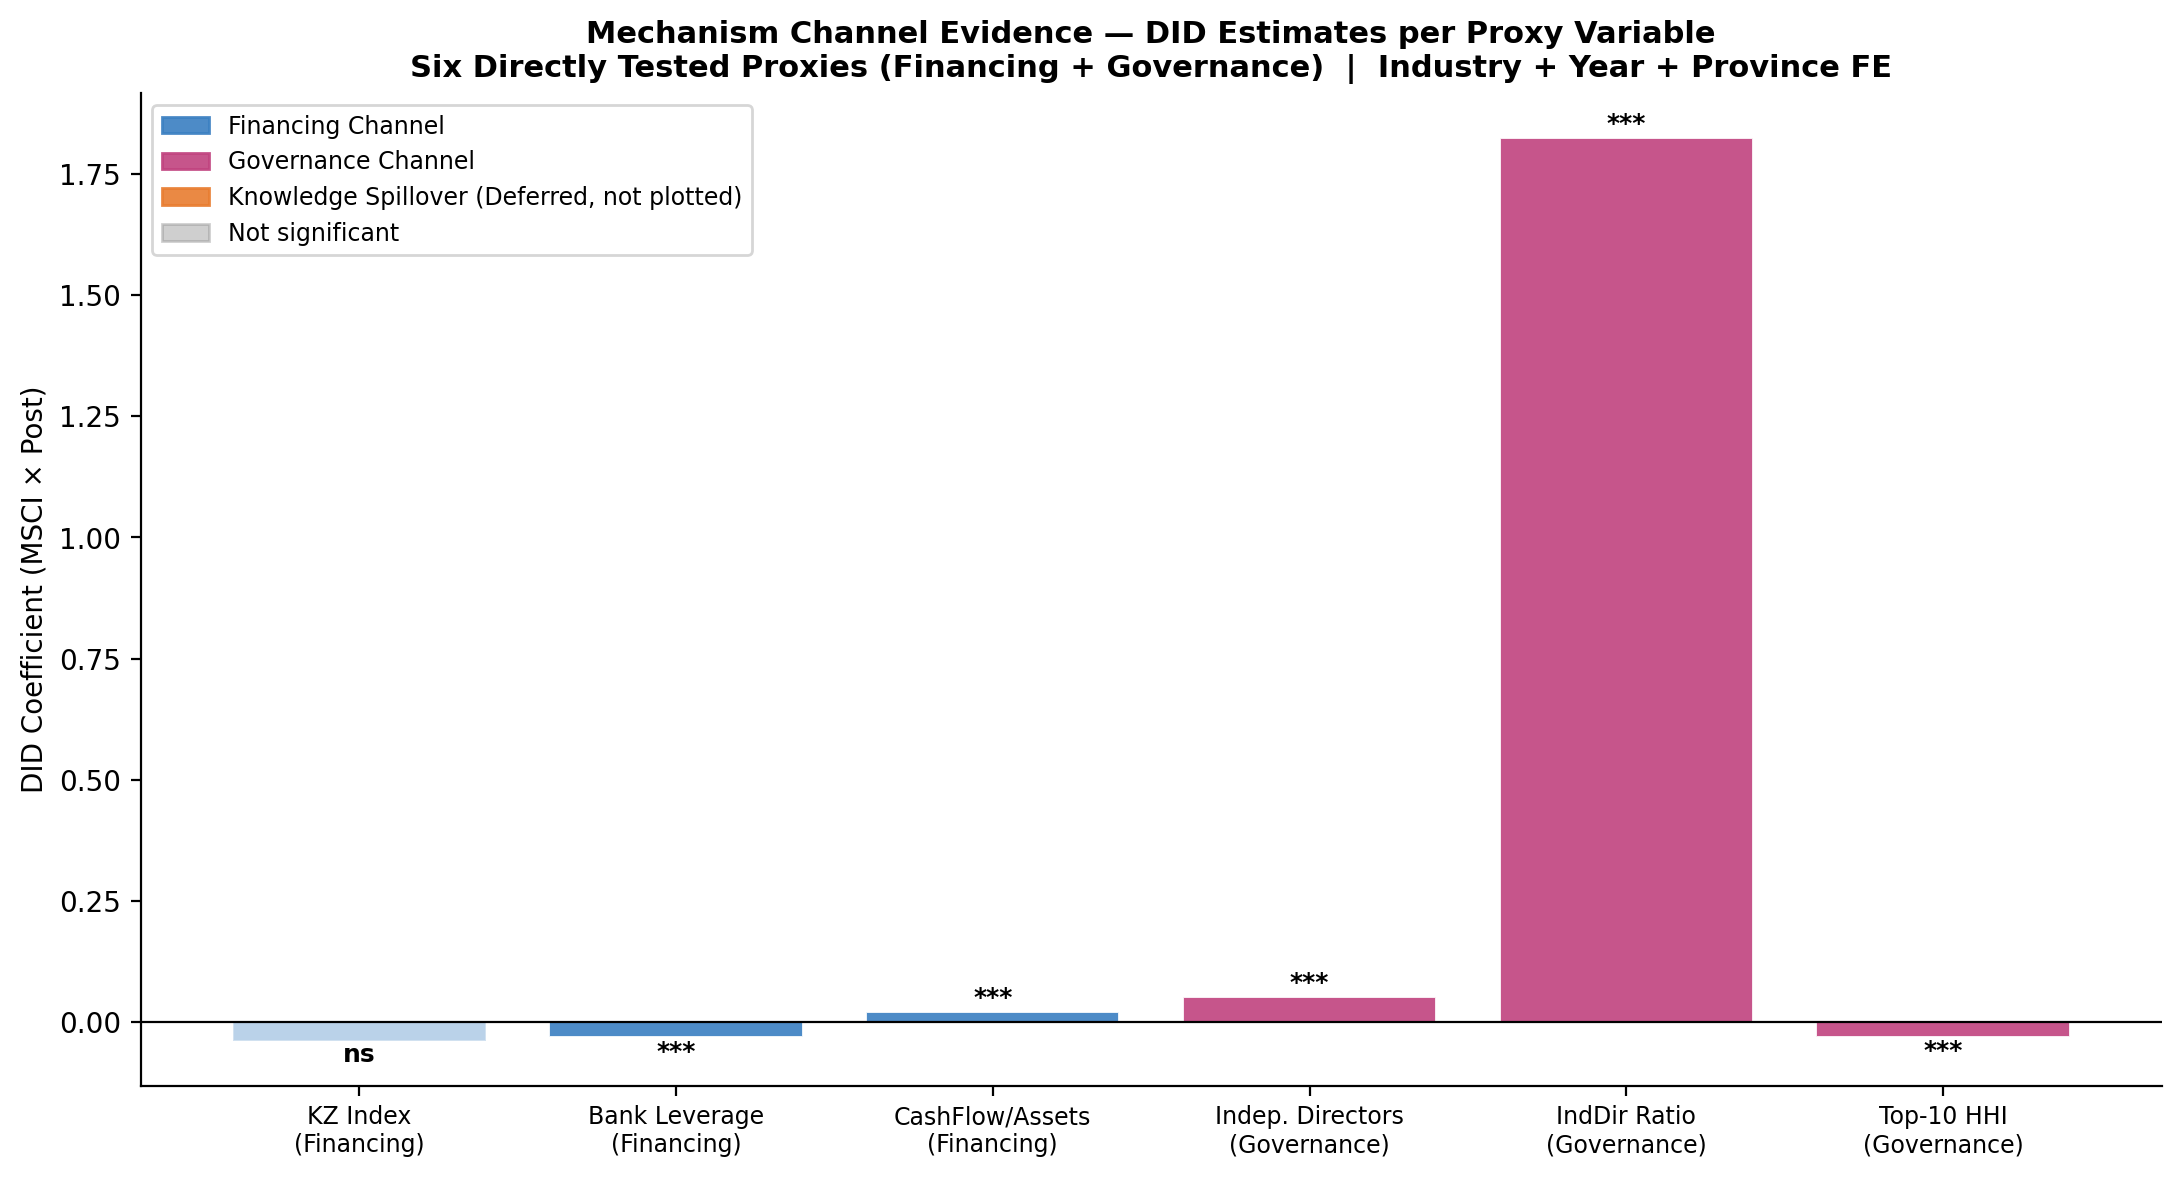
\includegraphics[width=0.90\textwidth]{figures/fig6_6_mechanism_channels.png}
\caption{Mechanism Channel Evidence: DID Estimates for Financing and Governance Proxies}
\label{fig:mechanism_channels}
\end{figure}

Figure~\ref{fig:mechanism_channels} presents the quantitative DID estimates for the six directly tested proxies in the financing and governance channels.

\subsection{Financing Constraint Channel: KZ Index, Bank Leverage, and Cashflow/Assets}

The financing-constraint channel predicts that MSCI inclusion lowers the effective cost of external capital for treated firms.

To make this channel operational, the thesis uses three complementary firm-year proxies with distinct measurement logic. KZ Index is treated as a composite financing-friction score where larger values indicate tighter constraints. Bank Leverage is the bank-debt reliance ratio in the merged panel (scaled by firm size), so lower values indicate reduced dependence on bank credit after treatment. CashFlow/Assets is operating cash flow scaled by total assets and captures internally generated liquidity available for digital investment. All three mechanism regressions retain the same identification structure as the baseline model (Industry+Year+Province fixed effects with firm-clustered standard errors), so channel coefficients remain directly comparable to the main DID specification.

\begin{table}[htbp]
\centering
\caption{Mechanism Analysis: Financing Channel}
\label{tab:financing_channel}
\small
\begin{tabular}{lccc}
\toprule
\textbf{Variable} & \textbf{(1) KZ Index} & \textbf{(2) Bank Leverage} & \textbf{(3) CashFlow/Assets} \\
\midrule
MSCI $\times$ Post & $-$0.0385 (0.0733) & $-$0.0318*** (0.0027) & 0.0201*** (0.0035) \\
Controls & Yes & Yes & Yes \\
Industry-FE & Yes & Yes & Yes \\
Year-FE & Yes & Yes & Yes \\
Province-FE & Yes & Yes & Yes \\
$N$ & 28,339 & 23,552 & 34,770 \\
\bottomrule
\end{tabular}
\begin{tablenotes}
\small
\item \textit{Notes:} Entries report MSCI $\times$ Post coefficients with firm-clustered standard errors in parentheses. $N$ varies by proxy due to data availability in CSMAR. Significance: *** $p < 0.01$, ** $p < 0.05$, * $p < 0.10$.
\end{tablenotes}
\end{table}

The financing estimates show a coherent pattern once variable scaling is considered. The KZ coefficient is negative ($-$0.0385) but imprecise (SE $=0.0733$, $p = 0.599$), so the composite index does not move significantly in this sample. In contrast, Bank Leverage declines significantly ($-$0.0318***, $p < 0.001$), equivalent to about a 3.2 percentage-point decline in bank-debt reliance. CashFlow/Assets increases by 0.0201*** ($p < 0.001$), or roughly a 2.0 percentage-point rise in internal funding capacity. The divergence between the noisy composite index and the precise balance-sheet proxies is informative rather than inconsistent: financing relief appears strongest on directly measured funding margins.

\subsection{Governance Channel: Independent Directors and Top-10 Ownership HHI}

International institutional investors are documented advocates of governance reform as a condition of sustained capital allocation~\cite{Aggarwal2011}.

This channel is measured using board-structure and ownership-concentration variables that map directly to monitoring intensity. $N$(Independent Directors) is the count of independent directors and captures board monitoring capacity in levels. Independent Director Ratio (\%) scales independent-director seats by total board size, so it captures compositional independence rather than board expansion alone. Top-10 Ownership HHI is a Herfindahl-type concentration index over top-shareholder holdings; larger values indicate tighter control concentration, while smaller values indicate more dispersed monitoring rights. Estimation again uses the same DID framework and fixed-effect structure as the baseline model, ensuring interpretation consistency across channels.

\begin{table}[htbp]
\centering
\caption{Mechanism Analysis: Governance Channel}
\label{tab:governance_channel}
\small
\begin{tabular}{lccc}
\toprule
\textbf{Variable} & \textbf{(1) Indep. Dir. Count} & \textbf{(2) Indep. Dir. Ratio} & \textbf{(3) Top-10 HHI} \\
\midrule
MSCI $\times$ Post & 0.0518*** (0.0152) & 1.8238*** (0.5627) & $-$0.0302*** (0.0054) \\
Controls & Yes & Yes & Yes \\
Industry-FE & Yes & Yes & Yes \\
Year-FE & Yes & Yes & Yes \\
Province-FE & Yes & Yes & Yes \\
$N$ & 26,522 & 20,136 & 34,753 \\
\bottomrule
\end{tabular}
\begin{tablenotes}
\small
\item \textit{Notes:} Entries report MSCI $\times$ Post coefficients with firm-clustered standard errors in parentheses. The HHI coefficient is expected to be negative if governance improves through ownership dispersion. Significance: *** $p < 0.01$, ** $p < 0.05$, * $p < 0.10$.
\end{tablenotes}
\end{table}

Governance estimates are uniformly in the predicted direction and statistically significant. MSCI-included firms add independent directors ($+$0.0518***, $p = 0.0007$). Although the annual increment per firm is modest, the estimate is precise in a large sample ($N=26{,}522$). More importantly, the independent-director ratio rises by 1.8238 percentage points ($p = 0.0012$), indicating compositional strengthening rather than simple board expansion. Top-10 Ownership HHI declines ($-$0.0302***, $p < 0.001$), consistent with ownership dispersion and broader minority-shareholder monitoring scope. Taken together, these proxies provide convergent evidence that the governance channel is statistically robust and economically meaningful.

\subsection{Knowledge Spillover Channel: Deferred Direct Test and Data Requirements}

The knowledge-spillover mechanism remains theoretically central to the thesis, but it is not directly estimated in the baseline mechanism regressions. Recent evidence shows that digital transformation can generate information spillovers across firms and market participants~\cite{WangWang2026}, and that spillover intensity may vary with strategic competition conditions in manufacturing settings~\cite{LiuGu2026}, reinforcing the conceptual relevance of this channel in our setting. A direct mechanism test requires mediator variables that map to the chain MSCI inclusion $\to$ external information intermediaries/investors $\to$ firm learning and implementation. In this context, analyst coverage (and optionally analyst forecast dispersion) and foreign institutional ownership are the preferred first-stage mediators. Because these variables are not yet integrated into the current merged panel, this thesis does not report a direct knowledge-channel coefficient and avoids proxy substitution that could blur causal interpretation.

For transparency, the intended measurement protocol is as follows: analyst coverage is defined as the number of analysts issuing firm-year forecasts; analyst forecast dispersion is the cross-analyst standard deviation of earnings forecasts; foreign institutional ownership is the fraction of shares held by foreign institutions in each firm-year; and cross-border exposure proxies include export intensity, overseas subsidiary presence, and foreign director participation. These variables are conceptually close to the mechanism chain and therefore preferred over indirect substitutes. As a supplementary check, Appendix Table~\ref{tab:appendix_spillover_proxy} reports an exploratory peer-spillover proxy regression based on leave-one-out industry-year peer digitalization. The interaction term (MSCI $\times$ PeerDT) is positive but statistically insignificant ($p = 0.114$), so it is reported only as directional context rather than direct mechanism evidence. The deferred design choice is methodological rather than substantive: the thesis prioritizes identification quality by reporting no direct-mediator coefficient instead of reporting a weakly interpretable proxy-based estimate.

To maintain analytical transparency for this deferred channel, Table~\ref{tab:knowledge_deferred} reports a structured measurement and identification roadmap rather than a placeholder pseudo-regression.

\begin{table}[!htbp]
\centering
\caption{Knowledge Spillover Channel: Direct-Test Data and Identification Requirements}
\label{tab:knowledge_deferred}
\small
\setlength{\tabcolsep}{4pt}
\begin{tabularx}{\textwidth}{>{\raggedright\arraybackslash}X>{\raggedright\arraybackslash}X>{\centering\arraybackslash}m{1.7cm}>{\raggedright\arraybackslash}X>{\centering\arraybackslash}m{2.0cm}>{\raggedright\arraybackslash}X}
\toprule
\textbf{Mediator (Preferred)} & \textbf{Mechanism Mapping} & \textbf{Expected Sign} & \textbf{Candidate Data Source} & \textbf{Current Status} & \textbf{Planned Empirical Test} \\
\midrule
Analyst coverage (and optionally analyst forecast dispersion) & MSCI inclusion $\to$ external information production $\to$ firm learning and implementation & $+$ (coverage), $-$ (dispersion) & CSMAR analyst module / CNRDS analyst files & Not yet merged & DID and event-study on mediator; mediation-consistency test with digital-transformation outcomes \\
Foreign institutional ownership share & MSCI inclusion $\to$ foreign monitoring and benchmarking pressure $\to$ managerial upgrading & $+$ & CSMAR ownership module / WIND foreign holding data & Not yet merged & DID on ownership response; interaction and mechanism regressions with firm and year FE \\
Cross-border exposure proxies (exports, overseas subsidiaries, foreign directors) & MSCI inclusion $\to$ global network exposure $\to$ knowledge diffusion & $+$ & CSMAR segment/disclosure modules; annual-report hand-collected fields & Partially available, not harmonized & Supplementary mechanism test after variable harmonization and missing-data diagnostics \\
\bottomrule
\end{tabularx}
\begin{tablenotes}
\small
\item \textit{Notes:} This table specifies the mediator architecture for the knowledge-spillover channel, including variable definitions, expected effect directions, candidate data sources, and planned empirical tests. Presenting the design at this stage preserves causal coherence while direct mediator series are being harmonized in the merged panel.
\end{tablenotes}
\end{table}

The row-by-row design in Table~\ref{tab:knowledge_deferred} clarifies what is missing and why. Analyst variables identify the information-production margin, foreign ownership identifies monitoring and benchmarking pressure, and cross-border exposure identifies network-based diffusion. Reporting these rows explicitly improves interpretability relative to an ``NA'' coefficient table because it links each mediator to a concrete data source, expected sign, and planned test design.

Taken together, Section~6.5 provides direct mechanism evidence for financing and governance channels. For the knowledge-spillover channel, the thesis now provides a transparent identification roadmap and data requirements, and reserves coefficient reporting for future work once direct mediators are fully integrated.

\paragraph{Cross-Channel Summary}

To synthesize mechanism evidence without conflating unlike units, Table~\ref{tab:cross_channel} reports sign, precision, and sample coverage across channels under a common fixed-effect specification.

\begin{table}[htbp]
\centering
\caption{Mechanism Analysis: Cross-Channel Summary}
\label{tab:cross_channel}
\small
\begin{tabular}{llcccc}
\toprule
\textbf{Channel} & \textbf{Variable} & \textbf{Coeff.} & \textbf{SE} & \textbf{$p$-val} & \textbf{$N$} \\
\midrule
Financing & KZ Index & $-$0.0385 & 0.0733 & 0.5992 & 28,339 \\
Financing & Bank Leverage & $-$0.0318*** & 0.0027 & 0.000 & 23,552 \\
Financing & CashFlow / Assets & 0.0201*** & 0.0035 & 0.000 & 34,770 \\
Governance & $N$(Indep.\ Directors) & 0.0518*** & 0.0152 & 0.0007 & 26,522 \\
Governance & Indep.\ Director Ratio (\%) & 1.8238*** & 0.5627 & 0.0012 & 20,136 \\
Governance & Top-10 Ownership HHI & $-$0.0302*** & 0.0054 & 0.000 & 34,753 \\
Knowledge (Deferred) & Direct mediators pending integration & -- & -- & -- & -- \\
\bottomrule
\end{tabular}
\begin{tablenotes}
\small
\item \textit{Notes:} All reported coefficients come from regressions with Industry+Year+Province FE and firm-clustered standard errors. Across the six directly tested proxies, five are significant at the 1\% level and all are directionally consistent with theory. The deferred knowledge row is a status indicator, not a regression estimate.
\end{tablenotes}
\end{table}

Table~\ref{tab:cross_channel} shows a clear ranking in empirical strength. In financing, two of three proxies are significant and both indicate easing of funding constraints through lower bank-debt reliance and higher internal liquidity, while the composite KZ index remains imprecise. In governance, all three proxies are significant and theory-consistent, making governance the most robust mechanism block in this sample. The deferred knowledge row is deliberately non-estimated and should be interpreted as a data-integration status marker rather than a null mechanism finding.

\section{Discussion}

This section integrates the evidence into a coherent interpretive framework and discusses implications for theory, methodology, and policy.

\subsection{Interpretation of Main Findings in Theoretical Context}

The 0.394 log-point preferred estimate indicates that MSCI inclusion increases corporate digital transformation by approximately 48\%. This magnitude is economically significant---corresponding to half a within-firm standard deviation and a multiple of the control group's 4\% organic annual growth rate---and directionally consistent with the theoretical framework in Chapter~\ref{chap:literature_review}. Mechanism evidence in Section~6.5 is strongest for governance (3/3 proxies significant), with supportive but mixed precision in financing (2/3 proxies significant).

The heterogeneity patterns---stronger effects in eastern provinces, technology-intensive industries, and high-end manufacturing subsectors---are consistent with an absorptive-capacity framework. International capital and knowledge flows appear to generate the largest digital-transformation returns where complementary institutional, human-capital, and technological resources are already in place.

\subsection{Implications for the Capital Market Liberalization Literature}

This study extends the capital market liberalization literature in three ways. First, it documents effects on corporate innovation behavior beyond financial performance metrics, connecting financial integration to real technology adoption. Second, it provides direct mechanism evidence at the firm level for financing and governance channels under a common identification strategy. Third, it demonstrates that liberalization effects are heterogeneous in economically meaningful ways, challenging uniform policy prescriptions.

\subsection{Implications for the Digital Transformation and Computational Economics Literature}

By combining validated text-as-data measures with a well-identified quasi-experiment, this study demonstrates that causal inference on digital-transformation drivers is feasible at scale in emerging markets. The consistency of results across eight alternative outcome measures further supports computational text analysis as a reliable approach for studying corporate innovation.

\subsection{Policy Implications for Regulators, Firms, and International Investors}

Several policy implications emerge. For policymakers, carefully sequenced capital market liberalization can produce technology-upgrading spillovers in addition to conventional market-efficiency gains. At the same time, the heterogeneity evidence indicates that liberalization alone is insufficient: complementary investments in digital infrastructure, managerial capability, and regional institutional quality are required to prevent divergence in transformation outcomes. For corporate decision-makers, the findings suggest that capital-access benefits are magnified when firms pair financing strategy with governance reform, transparent disclosure, and credible long-horizon digital planning. For international investors, results indicate that stewardship and monitoring functions can be active channels through which portfolio allocation influences real firm behavior.
